\documentclass{article}
\usepackage[utf8]{inputenc}
\usepackage{amsmath,amsfonts,amssymb,amsthm}
\usepackage{graphicx}
\usepackage{url}
\usepackage{hyperref}
\usepackage{xcolor}
\usepackage{booktabs}
\usepackage{multirow}
\usepackage[margin=1in]{geometry}
\usepackage{float}
\usepackage{natbib}

\newcommand{\software}[1]{\texttt{#1}}

\newtheorem{theorem}{Theorem}[section]
\newtheorem{proposition}{Proposition}[section]
\newtheorem{remark}{Remark}[section]

\title{Simulation-Based Power Calculation and Study Design for Circadian Rhythmic Analysis}
\author{}
\date{}

\begin{document}

\maketitle

\begin{abstract}
Circadian disruption is a hallmark of numerous human diseases, yet detecting condition-specific changes in gene expression rhythms remains a significant challenge. Circadian transcriptomic studies aim to identify rhythmic biomarkers within a given condition or to characterize differential circadian biomarkers across conditions. Given the constraints of limited budgets and sample availability, rigorous power calculation and thoughtful study design are critical for planning such studies. Existing approaches, such as CircaPower, offer closed-form analytical solutions for circadian biomarker detection but do not account for gene-specific signal-to-noise ratios or genome-wide false discovery. To address these limitations, we present SCP (Simulation-based Circadian Power), a versatile simulation-based framework for the study design of circadian transcriptomic analyses. Leveraging gene-specific information from pilot or publicly available data, SCP enables realistic, scientifically driven and statistically principled power calculations with false discovery rate (FDR) control. The framework supports sample size determination for circadian biomarker detection and accommodates multi-faceted differential rhythm analyses, including differential rhythmicity, differential phase, and differential MESOR. We further investigate the optimal balance between sampling frequency and biological replicates under budget constraints when active experimental design — such as in animal studies — is feasible. Additionally, a bootstrap procedure is introduced to quantify uncertainty in power curves and sample size recommendations. SCP is evaluated through extensive simulations and real data analyses, demonstrating strong performance for realistic and principled study design in circadian transcriptomics.
\end{abstract}
%% ====================================================================
\section{Introduction}

Circadian rhythms, endogenous $\sim$24-hour oscillations, play a fundamental role in physiology and disease \citep{takahashi2017transcriptional}. Disruption of circadian timing has been implicated in aging and neuropsychiatric disorders \citep{chen2016aging}, and rhythmic transcription regulates metabolism, synaptic function, and immune signaling \citep{takahashi2017transcriptional,mure2018diurnal,chen2016aging}. To unveil circadian regulation in transcriptomic data, studies generally pursue one of two goals: detecting potential circadian biomarkers within a single condition or characterizing differences in rhythmic patterns across conditions, including differential rhythmicity (DR), differential phase (DP), and differential MESOR (i.e., rhythm-adjusted mean expression) (DM). A growing number of methods have been developed for both settings, including rhythmicity detection methods such as \textsc{JTK\_CYCLE}, \textsc{RAIN}, and \textsc{BIO\_CYCLE} for single-condition studies \citep{Hughes2010jtkcycle,Thaben2014rain,Agostinelli2016biocycle}, and differential frameworks such as \textsc{CircaCompare}, \textsc{LimoRhyde}, and \textsc{DiffCircaPipeline} for cross-condition analysis \citep{parsons2020circacompare,Singer2019LimoRhyde,xue2023diffcircapipeline}. While these methods enable statistical inference on circadian signals, they do not address how studies should be designed to achieve reliable detection.

Prospective study design therefore remains a critical bottleneck. Investigators must determine the sample size required to achieve adequate statistical power, assess how sensitive those recommendations are to the limitations of pilot data, and — in active experimental designs — strike the right balance between sampling frequency and biological replicates. In passive observational settings, such as human post-mortem studies, sampling time cannot be controlled and sample acquisition is costly, making principled sample size calculation especially important. Without rigorous design guidance, circadian transcriptomic studies risk being substantially underpowered despite considerable experimental investment.

To our knowledge, \textsc{CircaPower} \citep{zong2023circapower} is currently the only dedicated framework for power and sample size determination in circadian transcriptomic studies. However, it is restricted to single-condition rhythmicity detection and does not extend to differential rhythmicity analysis. CircaPower derives closed-form power calculations under a cosinor model using a fixed intrinsic effect size \( r = A/\sigma \), quantifying per-gene statistical power for detecting rhythmicity. While this provides an important statistical foundation for circadian biomarker discovery, the formulation assumes a uniform effect size across genes and does not account for genome-wide false discovery. In practice, however, the intrinsic effect size \( r \) varies substantially across tissues, species, and genes, with marked differences between core clock genes and the broader transcriptome \citep{zong2023circapower}. Consequently, the fixed-effect-size assumption fails to capture the heterogeneity in signal strength across the genome. Furthermore, because circadian studies operate at the transcriptome-wide scale, false discovery rate (FDR) control is essential. The fixed-\( r \) formulation does not naturally accommodate this requirement, as it lacks a mechanism to model cross-gene variability — a necessary ingredient for characterizing genome-wide error rates.

For power calculation of differential circadian biomarker detection, closed-form analytical solutions analogous to those in CircaPower are generally infeasible. As established in DiffCircaPipeline \citep{xue2023diffcircapipeline}, circadian rhythm disruptions are complex and multi-faceted, encompassing differential rhythmicity (DR), differential phase (DP), and differential MESOR (DM). Detection of these features requires a two-stage workflow contingent on the rhythmicity status inferred for each condition. From a statistical standpoint, this biological complexity involves multiple endpoints coupled with genome-wide multiple testing, and therefore cannot be reduced to a single test statistic or a tractable closed-form solution.

These gaps motivate the development of \textbf{SCP} (Simulation-based Circadian Power), a simulation-based framework for power calculation and study design that supports practical decision-making in planning circadian transcriptomic studies. Section \ref{sec:single_cohort} presents power calculation for circadian biomarker detection in a single cohort, incorporating gene-specific information from pilot data and controlling for FDR. Section \ref{sec:differential} addresses power calculation for multi-faceted differential circadian analysis in a case-control setting. Section \ref{sec:active_design} provides guidance on optimizing the trade-off between sampling frequency and biological replicates under budget constraints. Section \ref{sec:bootstrap} introduces a bootstrap procedure to quantify uncertainty in power estimates and sample size recommendations, which is particularly valuable when pilot data exhibit weak signal. Section \ref{sec:results} presents extensive simulation studies and real data analyses benchmarking the performance of SCP across a range of realistic settings. Together, these components combine analytical efficiency with simulation-based flexibility, equipping researchers with a principled and practical framework for designing circadian transcriptomic studies.

%% ====================================================================
% =====================================================================
% SCP METHODS SECTION — REVISED DRAFT
% Changes are annotated with % CHANGE: comments explaining each edit.
% =====================================================================

\section{Methods}



% =====================================================================
\subsection{Power calculation for circadian biomarker detection in single cohort}
\label{sec:single_cohort}

For a single cohort of $n$ subjects with sample collection time-of-day (TOD)
$t_1,\ldots,t_n\in[0,24)$, the expression of gene $g$ follows the cosinor model
\begin{equation}
y_{gi}
=
\mu_g
+
A_g\cos \bigl(\omega(t_i - \phi_g)\bigr)
+
\varepsilon_{gi},
\qquad
\varepsilon_{gi}\overset{\text{iid}}{\sim}N(0,\sigma_g^2),
\label{eq:cosinor_model}
\end{equation}
where $\omega=2\pi/24$, $\mu_g$ is the MESOR (Midline Estimating Statistic Of Rhythm; i.e., rhythm-adjusted mean expression), $A_g\geq 0$ is the amplitude,
$\phi_g\in[0,24)$ is the acrophase, and $\sigma_g$ is the noise level. The CircaPower paper by Zong et al. \cite{zong2023circapower} established the theoretical foundations of power calculation of circadian biomarker detection below under the cosinor model with Gaussian errors. To test for rhythmicity of gene $g$, $F$-statistic for $H_0: A_g = 0$ versus $H_A: A_g > 0$ was considered: 
\begin{equation}
F_g
=
\frac{(\mathrm{TSS}_g - \mathrm{RSS}_g)/2}{\mathrm{RSS}_g/(n-3)}
\sim F(2,\, n-3),
\label{eq:rhythm_f_test}
\end{equation}
where $\mathrm{RSS}_g$ and $\mathrm{TSS}_g$ are the residual and total sums of
squares from the cosinor fit and $F(a,\, b)$ is F-distribution with degrees of freedom $a$ and $b$. Across $G$ genes, Benjamini--Hochberg (BH)
correction at nominal FDR level $\alpha$ controls FDR for rhythmicity detection.

For power calculation, under the alternative hypothesis $H_A$, the $F$-statistic follows a noncentral $F$-distribution:
$F_g\sim  F\bigl( 2,\, n-3, \, \lambda_g\bigr)$ with degrees of freedom $2$ and $n-3$ and noncentrality parameter $\lambda_g$. The per-gene statistical power at sample size $n$ is then
\begin{equation}
\mathrm{Power}_g(n)
=
1 - F\bigl(q_{\alpha}; 2,\, n-3, \, \lambda_g\bigr),
\label{eq:circapower_formula}
\end{equation}

\noindent where $q_{\alpha}=F(1-\alpha;\,2,\,n-3)$ is the rejection threshold under $H_0$ at level $\alpha$ and $F(x; a,b)$ is the CDF of F-distribution $F(2, n-3)$; $F(x; a,b,\lambda)$ is the CDF of noncentral F-distribution $F(a,b,\lambda)$. 

Zong et al.(2024) showed that 
\begin{equation}
\lambda_g = r_g^2 \cdot n \cdot d(\phi_g),
\label{eq:ncp}
\end{equation}
where $r_g = A_g/\sigma_g$ is the intrinsic effect size of gene $g$, and the design factor $d(\phi_g)$ captures how well the sample collection TOD $(t_1,\cdots, t_n)$ spread on time domain:
\begin{equation}
d(\phi_g)
=
\frac{1}{n}\sum_{i=1}^n \cos^2\bigl(\omega(t_i - \phi_g)\bigr)
-
\left(\frac{1}{n}\sum_{i=1}^n \cos\bigl(\omega(t_i - \phi_g)\bigr)\right)^{\!2}.
\label{eq:design_factor_circapower}
\end{equation}

% CHANGE: Moved B-invariance note here as a brief statement with a forward
% pointer, removing the mid-paragraph digression. Full derivation is reserved
% for Section~\ref{sec:active_design} and Supplementary~S8.
For balanced equally spaced active designs with $B\geq 3$ time points,
$d(\phi_g)=1/2$ for all phases, so \eqref{eq:ncp} reduces to
$\lambda_g = r_g^2 n / 2$ and power depends only on $r_g$ and $n$; see
Section~\ref{sec:active_design} and Supplementary~S8.

In transcriptome-wide studies, however, $r_g$ varies substantially across
genes: core clock genes in mouse liver typically have $r \approx 3$--$6$,
while the median $r$ across all expressed genes in human brain tissue is
$\tilde{r}\approx 0.6$ \citep{zong2023circapower}.


Using a single representative $r$, as in \textsc{CircaPower}, therefore produces
severely over-optimistic power projections for the majority of the transcriptome,
and the per-gene formula \eqref{eq:circapower_formula} does not account for the
multiple-testing correction applied when testing thousands of genes simultaneously.
\textsc{SCP} addresses these limitations through the following four-step
simulation pipeline.



\emph{Step 1 --- Pilot parameter estimation.}
For each of the $G_0$ pilot genes, fit \eqref{eq:cosinor_model} by OLS to obtain
$(\hat{\mu}_g, \hat{A}_g, \hat{\sigma}_g, \hat{\phi}_g)$ and the corresponding
$p$-value $p_g$ for rhythmicity. To improve stability across datasets with
heterogeneous signal strength, we define a pilot-stage screening rule based on
a fixed marginal threshold $\alpha_{\text{pilot}}$ (default $\alpha_{\text{pilot}}=0.01$),
rather than using multiplicity-adjusted thresholds. Let
$\mathcal{G}_R^{\mathrm{cand}} = \{g : p_g < \alpha_{\text{pilot}}\}$ and
$K = \min\bigl(300,\ |\mathcal{G}_R^{\mathrm{cand}}|\bigr)$, and define the
parameter-estimation set as the top-ranked genes
$\mathcal{G}_R = \mathrm{Top}_K(\mathcal{G}_R^{\mathrm{cand}})$.
The estimated rhythmic proportion is given by
$\hat{\pi}_R = |\mathcal{G}_R^{\mathrm{cand}}| / G_0$.
Empirical distributions are then constructed over the fitted parameters:
\begin{equation}
\hat{F}_\mu
=
\frac{1}{G_0}\sum_{g=1}^{G_0}\delta_{\hat{\mu}_g},
\quad
\hat{F}_{A,\sigma}
=
\frac{1}{|\mathcal{G}_R|}\sum_{g\in\mathcal{G}_R}\delta_{(\hat{A}_g,\hat{\sigma}_g)},
\quad
\hat{F}_{\phi}
=
\frac{1}{|\mathcal{G}_R|}\sum_{g\in\mathcal{G}_R}\delta_{\hat{\phi}_g}.
\label{eq:empirical_dists}
\end{equation}
The mesor distribution $\hat{F}_\mu$ is estimated from all $G_0$ genes, reflecting a
shared baseline-expression level across the transcriptome regardless of rhythmic status.
We assume a shared empirical mesor distribution across genes, while allowing
gene-specific mesor shifts between groups under the DM state
(Section~\ref{sec:differential}).
Sampling $(A,\sigma)$ jointly from $\hat{F}_{A,\sigma}$ preserves the empirical
amplitude-noise dependence, so the induced
$r=A/\sigma$ distribution reflects this relationship without requiring $r$ to be specified separately.
The complete pilot summary $\hat{\Psi} = (\hat{F}_\mu, \hat{F}_{A,\sigma},
\hat{F}_\phi, \hat{F}_{\mathrm{TOD}}, \hat{\pi}_R)$ is passed to the downstream
steps, where $\hat{F}_{\mathrm{TOD}}$ is the empirical collection-time
distribution for passive designs. The choice of $\alpha_{\text{pilot}}$ can be
adjusted by the user.

\emph{Step 2 --- Data generation.}
For each simulation replicate $s=1,\ldots,S$ and candidate sample size $n$,
draw rhythmicity indicators $Z_{g,s}^R \sim \mathrm{Bernoulli}(\hat{\pi}_R)$
independently for $g=1,\ldots,G$. Conditional on $Z_{g,s}^R$, observations are
generated from a two-component mixture model
\[
y_{g,i}^{(s)} \mid Z_{g,s}^R \sim
\begin{cases}
M_1\!\left(\mu_g^{(s)}, A_g^{(s)}, \sigma_g^{(s)}, \phi_g^{(s)}\right), & Z_{g,s}^R = 1, \\[6pt]
M_0\!\left(\mu_g^{(s)}, \sigma_g^{(s)}\right), & Z_{g,s}^R = 0,
\end{cases}
\]
where the rhythmic model $M_1$ is the cosinor model
\[
M_1:\quad
y_{g,i}^{(s)} = \mu_g^{(s)} + A_g^{(s)} \cos\!\bigl(\omega t_i + \phi_g^{(s)}\bigr)
+ \varepsilon_{g,i}^{(s)}, \qquad
\varepsilon_{g,i}^{(s)} \sim \mathcal{N}\bigl(0, (\sigma_g^{(s)})^2\bigr),
\]
and the arrhythmic model $M_0$ is the reduced intercept-only model
\[
M_0:\quad
y_{g,i}^{(s)} = \mu_g^{(s)} + \varepsilon_{g,i}^{(s)}, \qquad
\varepsilon_{g,i}^{(s)} \sim \mathcal{N}\bigl(0, (\sigma_g^{(s)})^2\bigr).
\]

For genes with $Z_{g,s}^R=1$, parameters are sampled as
$\mu_g^{(s)}\sim\hat{F}_\mu$, $(A_g^{(s)},\sigma_g^{(s)})\sim\hat{F}_{A,\sigma}$,
and $\phi_g^{(s)}\sim\hat{F}_\phi$. For genes with $Z_{g,s}^R=0$, we set
$A_g^{(s)}=0$, sample $\mu_g^{(s)}\sim\hat{F}_\mu$, and sample $\sigma_g^{(s)}$
from the empirical marginal distribution of $\sigma$ implied by $\hat{F}_{A,\sigma}$.

An \emph{active} design specifies $B$ distinct time points with $m_b$ replicates
each and total $n=\sum_b m_b$; a \emph{passive} design draws collection times
from $\hat{F}_{\mathrm{TOD}}$. For balanced equally spaced active designs with
$B\geq 3$, $d(\phi)=1/2$ for all phases, so power depends only on total $n$;
for passive designs the realized $d(\phi_g)$ is computed from the observed
collection times via \eqref{eq:design_factor_circapower}, varies by gene and
replicate, and \textsc{SCP} reports design-factor diagnostics. 




\emph{Step 3 --- Inference.}
Apply the $F$-test \eqref{eq:rhythm_f_test} to every gene and BH correction at
nominal level $\alpha$ across all $G$ genes. Let $D_{g,s}\in\{0,1\}$ denote
the discovery indicator ($D_{g,s}=1$ if gene $g$ is declared rhythmic in
replicate $s$).

\emph{Step 4 --- Power aggregation.}
With $Z_{g,s}^R\in\{0,1\}$ the true rhythmicity status assigned in Step~2,
empirical power is
\[
\widehat{\mathrm{Power}}(n)
=
\frac{1}{S}\sum_{s=1}^S
\frac{\sum_g D_{g,s}Z_{g,s}^R}{\sum_g Z_{g,s}^R},
\]
and empirical FDR is the per-replicate fraction of false discoveries among all
discoveries, averaged across $S$ replicates. Because parameters are drawn from
the full pilot distributions $\hat{F}_\mu$, $\hat{F}_{A,\sigma}$, and $\hat{F}_\phi$
(Step~1), the power estimate integrates over the observed transcriptome-wide
heterogeneity in baseline expression, amplitude, noise, and phase rather than
relying on a single representative effect size. Because BH
correction is applied within each replicate (Step~3), genome-wide multiplicity
control is captured naturally rather than treated as a post-hoc adjustment.
The indicators $D_{g,s}$ and $Z_{g,s}^R$ introduced here carry over directly
to Section~\ref{sec:differential}, where endpoint-specific superscripts
distinguish among differential endpoints.

% CHANGE: CF shortcut paragraph moved here from its original mid-section
% location. Positioning it after Step 4 frames it naturally as an efficient
% alternative to the full pipeline, and the trade-off guidance is immediately
% visible rather than buried before the steps.

A computationally efficient alternative to the full simulation pipeline is also available for the single-cohort setting. Equation~\eqref{eq:circapower_formula}
is evaluated gene-by-gene at each pilot gene's estimated
$\hat{r}_g = \hat{A}_g/\hat{\sigma}_g$ and design factor
$\hat{d}(\hat{\phi}_g)$, and the results are averaged to yield
$\widehat{\mathrm{Power}}_{\mathrm{CF}}(n)$.
This approximation is computationally efficient, but it does not propagate
genome-wide FDR or the joint $(A_g,\sigma_g)$ heterogeneity. The full
simulation-based pipeline is therefore recommended when transcriptome-wide
operating characteristics are the primary design target.

\subsection{Power calculation for case-control differential circadian analysis}
\label{sec:differential}

The single-group indicators $D_{g,s}$ and $Z_{g,s}^R$ from
Section~\ref{sec:single_cohort} generalize to the two-group setting as follows.
For each endpoint $E\in\{\mathrm{DR},\mathrm{DP},\mathrm{DM}\}$,
$D_{g,s}^E\in\{0,1\}$ denotes the endpoint-specific discovery indicator and
$Z_{g,s}^E\in\{0,1\}$ denotes the true differential status. A targeted indicator $Z_{g,s}^{*,E} = Z_{g,s}^E \cdot \mathbf{1}\{\delta_{g,s}^E \geq \Delta_E\}$ restricts attention to genes whose effect size exceeds a user-specified threshold $\Delta_E$, where
$\delta_{g,s}^{\mathrm{DR}} = |R_{g,1,s}^2 - R_{g,2,s}^2|$ is the absolute difference in cosinor goodness-of-fit between groups,
$\delta_{g,s}^{\mathrm{DP}} = \min\!\bigl(|\phi_{g,1,s}-\phi_{g,2,s}|,\,24-|\phi_{g,1,s}-\phi_{g,2,s}|\bigr)$ is the circular phase distance,
and $\delta_{g,s}^{\mathrm{DM}} = |\mu_{g,2,s} - \mu_{g,1,s}|$ is the absolute mesor difference.

When comparing rhythmic patterns between two groups, inference becomes
multi-stage: genes are first partitioned by per-group rhythmicity, followed by
endpoint-specific tests within data-derived strata. Because the multi-stage inference procedure does not yield tractable analytical
expressions for power and FDR, these quantities are evaluated via simulation
following the full analysis pipeline.

\textsc{SCP} evaluates three endpoints: differential rhythmicity (DR), differential
phase (DP), and differential mesor (DM). DR captures gain or loss of rhythmicity
(e.g., clock genes that cycle in healthy tissue but lose rhythmicity in disease);
DP captures a shift in peak-expression timing; and DM captures a change in
baseline expression level while rhythmic structure is preserved.
Their simulation proportions are denoted
$(\pi_{\mathrm{DR}}, \pi_R, \pi_{\mathrm{DP}}, \pi_{\mathrm{DM}})$.
When pilot data for both groups are available, $\pi_{\mathrm{DR}}$ and
$\pi_{\mathrm{DP}}$ are estimated empirically from the two-group pilot comparison;
$\pi_{\mathrm{DM}}$ is always user-specified, as mesor differences are not reliably
identifiable from the pilot distributions used to calibrate baseline parameters.
Otherwise all proportions are user-specified, with $\pi_R$ initialized from
$\hat{\pi}_R$ by default. When group-specific pilot data are available, the shared
summary $\hat{\Psi}$ can be replaced by group-specific summaries
$\hat{\Psi}_1$ and $\hat{\Psi}_2$, each estimated from the corresponding pilot,
to capture group-level heterogeneity in baseline parameters.
The simulation follows the same four-step structure as
Section~\ref{sec:single_cohort}, with Step~1 shared.

\emph{Step 2 --- Two-group data generation.}
For each gene, a baseline parameter tuple
$(\mu_g^{(s)}, A_g^{(s)}, \sigma_g^{(s)}, \phi_g^{(s)})$
is sampled from the pilot summary
$\hat{\Psi}=(\hat{F}_{\mu},\hat{F}_{A,\sigma},\hat{F}_{\phi},\hat{F}_{\mathrm{TOD}})$
constructed in Step~1, with $\hat{F}_\mu$ estimated from all $G_0$ genes and
$\hat{F}_{A,\sigma}$, $\hat{F}_\phi$ from the rhythmic set $\mathcal{G}_R$.
A latent type $T_g \in \{0,1,2,3,4,5\}$ is then independently assigned by
sampling from a categorical distribution with probabilities determined by
$(\pi_{\mathrm{DR}}, \pi_R, \pi_{\mathrm{DP}}, \pi_{\mathrm{DM}})$, where
differential rhythmicity is split equally into loss ($T_g=2$) and gain ($T_g=3$).

Group-specific parameters are initialized by setting
$\mu_{g,1}^{(s)} = \mu_{g,2}^{(s)} = \mu_g^{(s)}$,
$A_{g,1}^{(s)} = A_{g,2}^{(s)} = A_g^{(s)}$, and
$\phi_{g,1}^{(s)} = \phi_{g,2}^{(s)} = \phi_g^{(s)}$, and are then modified
according to $T_g$. Observations are generated as
\[
y_{g,i,k}^{(s)} \sim M_{T_g}(\mu_{g,k}^{(s)}, A_{g,k}^{(s)}, \sigma_g^{(s)}, \phi_{g,k}^{(s)}),
\quad k\in\{1,2\},
\]
where $M_1$ denotes the cosinor model and $M_0$ the intercept-only model,
with Gaussian noise $\varepsilon_{g,i,k}^{(s)} \sim \mathcal{N}(0,(\sigma_g^{(s)})^2)$.

Specifically, $T_g=0$ yields arrhythmic genes with $A_{g,1}=A_{g,2}=0$ and
$y_{g,i,k}^{(s)}=\mu_g^{(s)}+\varepsilon_{g,i,k}^{(s)}$ (model $M_0$),
whereas $T_g=1$ yields jointly rhythmic genes with shared parameters across
groups following $M_1$. For differential rhythmicity, $T_g=2$ sets $A_{g,2}=0$
and $T_g=3$ sets $A_{g,1}=0$, so that one group follows $M_1$ and the other
$M_0$. For differential phase ($T_g=4$), both groups follow $M_1$ with
$\phi_{g,2} = (\phi_{g,1} + \Delta \phi_g)\bmod 24$ and
$\Delta \phi_g \sim \mathrm{Unif}(\Delta \phi_{\min}, \Delta \phi_{\max})$;
for differential mesor ($T_g=5$), both groups follow $M_1$ with
$\mu_{g,2} = \mu_{g,1} + \Delta \mu_g$ and
$\Delta \mu_g \sim \mathrm{Unif}(\Delta \mu_{\min}, \Delta \mu_{\max})$.

\emph{Step 3 --- DCP inference.}
Inference proceeds via \textsc{DiffCircaPipeline}. For each group $k$,
cosinor models are fit and $p$-values $p_{g,k}$ are obtained. Genes are
assigned TOJR labels:
\[
\hat{Z}_g =
\begin{cases}
\texttt{arrhy}   & p_{g,1}>\alpha \text{ and } p_{g,2}>\alpha,\\
\texttt{g1-only} & p_{g,1}\leq\alpha \text{ and } p_{g,2}>\alpha,\\
\texttt{g2-only} & p_{g,1}>\alpha \text{ and } p_{g,2}\leq\alpha,\\
\texttt{both}    & p_{g,1}\leq\alpha \text{ and } p_{g,2}\leq\alpha.
\end{cases}
\]
where $\alpha$ denotes the inference-stage threshold, distinct from the
pilot-stage threshold $\alpha_{\text{pilot}}$ used in Step~1. Endpoint-specific
tests are then applied within strata, followed by BH correction at level $\alpha$.

\emph{Step 4 --- Power and FDR summarization.}
For each endpoint $E$, let $R_s^E=\sum_g D_{g,s}^E$ and
$V_s^E=\sum_g D_{g,s}^E(1-Z_{g,s}^E)$. The per-replicate FDR is
$\widehat{\mathrm{FDR}}_s^E = V_s^E/R_s^E$ when $R_s^E>0$, and 0 otherwise.
Targeted power is
\begin{equation}
\widehat{\mathrm{TPower}}_s^E(\Delta_E)
=
\frac{\sum_g D_{g,s}^E Z_{g,s}^{*,E}}{\sum_g Z_{g,s}^{*,E}}.
\label{eq:tpower_def}
\end{equation}
Final summaries are obtained by averaging across simulation replicates.





\subsection{Active study design: sampling frequency and replication trade-off}
\label{sec:active_design}

In a balanced active design, total sample size satisfies $N = Bm$, where $B$
is the number of distinct sampling time points and $m = N/B$ is the number of
biological replicates per time point. The investigator must allocate a fixed
subject budget between temporal coverage ($\uparrow B$, $\downarrow m$) and
biological replication ($\downarrow B$, $\uparrow m$). This allocation has
historically been guided by convention: landmark transcriptomic studies sampled
every 2--4 hours ($B = 6$--$12$, $m = 1$--$2$), inheriting the resolution of
physiological locomotor recordings~\citep{[CITE]}, and the practice has
continued at scale without formal power justification~\citep{[CITE]}. No
existing tool evaluates the full $(B, m)$ allocation surface under the
detection method a researcher plans to use: \textsc{CircaPower}~\citep{zong2023circapower}
computes the analytical non-centrality parameter at a single $(B, N, r)$ point
but does not sweep the allocation, and closed-form power expressions are
unavailable for non-parametric tests (\textsc{JTK\_CYCLE}, \textsc{RAIN}). As
a result, design choices such as $B = 4, m = 12$ versus $B = 12, m = 4$ at
fixed budget can lead to materially different power, yet this tradeoff remains
invisible in current practice.

The fundamental reason is that detection methods differ in how they use the
$(B, m)$ allocation. For cosinor-based methods (\textsc{DCP}), under a
balanced, equally spaced, first-harmonic sinusoidal design with $B \geq 3$
($\alpha_2 = 0$), the non-centrality parameter for gene $g$ is
\begin{equation}
  \lambda_g \;=\; \frac{r_g^2\, N}{2},
  \label{eq:ncp_invariance}
\end{equation}
independent of the $(B, m)$ split (Section~\ref{sec:single_cohort};
Supplementary~S8). Under these assumptions, power is invariant to the
allocation at fixed $N$: practitioners using a cosinor-based test may choose
$B$ freely on biological or logistical grounds without sacrificing detection
power.

Non-parametric rank-based methods do not share this invariance.
\textsc{JTK\_CYCLE} computes a Jonckheere-Terpstra statistic by accumulating
$\binom{B}{2}$ pairwise Mann-Whitney comparisons across time-point groups. At
fixed $N$, increasing $B$ adds more timepoint pairs but shrinks the per-group
sample $m = N/B$, reducing rank evidence per comparison. Beyond this precision
loss, adjacent timepoints in a dense design are separated by only a small phase
angle, so the cosine difference between groups is small and contributes little
signal regardless of $m$. Power therefore depends non-monotonically on $B$,
with an empirical interior optimum near $B \approx 4$--$6$
(Section~\ref{sec:bvsm_results}). \textsc{RAIN}'s umbrella test has
qualitatively similar $B$-sensitivity. As an extension explored in this work, we also evaluate an adaptive
multi-harmonic detector (\textsc{MH}), which fits a truncated Fourier model
with $K = \lfloor (B-1)/2 \rfloor$ harmonics and selects $K$ based on the
design. This method follows a distinct logic: a $K$-harmonic model requires
$B \geq 2K + 1$ equally-spaced observations for identifiability, so denser
sampling directly enables detection of higher-order waveform components when
$\alpha_2 > 0$. Thus, unlike cosinor-based methods, increasing $B$ is not
merely a reallocation choice for \textsc{MH}; it changes the class of
waveforms that can be estimated.

The practical consequence scales with signal strength. At high effect sizes
($\tilde{r} \gtrsim 2$, typical of mouse liver or lung), power saturates
rapidly with $N$ across all methods and $B$ choices, and the allocation is
largely inconsequential. At low to moderate effect sizes ($\tilde{r} \lesssim
1$, as in human post-mortem brain or cell-type-resolved preparations), the
method--$B$ interaction can substantially change detection power, and in some
settings by more than 20 percentage points. This is precisely the scenario
where principled design guidance is most critical. \textsc{SCP} addresses this
by sweeping the full $(N, B, \mathrm{method}, \alpha_2)$ grid on pilot data,
producing joint power surfaces that make the allocation tradeoff explicit for
each study context (Section~\ref{sec:bvsm_results}).

\paragraph{Active design under cosinor vs.\ FMM truth.}
The $B$-invariance result \eqref{eq:ncp_invariance} is derived under the
cosinor data-generating model. When the underlying truth is non-sinusoidal
(realistic per Section~\ref{sec:fmm_robustness}), denser temporal sampling
(higher $B$) better captures the asymmetric peak shape, and the trade-off
becomes non-trivial. We therefore evaluate the $(N, B)$ grid under both
truth conditions: (i) cosinor truth ($\omega = 1$, $\alpha = 0$), where
power is approximately flat across $B$ at fixed $N$; and (ii) empirical
FMM truth, where per-gene $(\hat A_g, \hat\sigma_g, \hat\phi_g, \hat\omega_g,
\hat\alpha_g)$ are drawn jointly from the same pilot gene index, preserving
the empirical $(A, \sigma, \omega, \alpha)$ correlations. The contrast
between the two rows in Fig~\ref{fig:active_vs_passive} quantifies how
much the cosinor approximation costs in design-sensitivity at the elbow
of the power curve.

% =====================================================================
\subsection{Robustness of DCP power to non-sinusoidal waveforms}
\label{sec:fmm_robustness}

\paragraph{Motivation.}
The cosinor model $M_1$ assumes a pure sinusoidal waveform. Real circadian
gene expression profiles can be asymmetric or sharply peaked, departing from
this ideal. A natural question is therefore how much power \textsc{DCP} loses
when the true waveform is non-sinusoidal. We quantify this loss by generating
data from a parametric family that nests the cosinor as a limiting case,
then applying the unmodified \textsc{DCP} test.

\paragraph{Violation model.}
As the data-generating process for the non-sinusoidal scenario we use the
Frequency Modulated M\"{o}bius (FMM) model of \citet{rueda2019fmm}:
\begin{equation}
y_{gi}
=
\mu_g
+
A_g\cos\!\bigl(\beta + 2\arctan\!\bigl(\omega^*\tan\tfrac{t_i-\phi_g}{2}\bigr)\bigr)
+
\varepsilon_{gi},
\qquad
\varepsilon_{gi}\overset{\text{iid}}{\sim}N(0,\sigma_g^2),
\label{eq:fmm_model}
\end{equation}
where $\omega^*\in(0,1]$ is the \emph{shape parameter} and $\beta\in[0,2\pi)$
is the \emph{orientation parameter}. This family is suited to the robustness
question for three reasons. First, at $\omega^*=1$, applying the identity
$2\arctan(\tan(x/2))=x$ reduces \eqref{eq:fmm_model} exactly to the cosinor
model \eqref{eq:cosinor_model} with acrophase $\phi_g = \alpha_g - \beta$;
decreasing $\omega^*$ continuously deforms the waveform from a pure sinusoid
toward increasingly peaked and asymmetric shapes, so the degree of violation
is controlled by a single interpretable parameter. Second, FMM is a
well-studied parametric family with biologically interpretable parameters
validated on circadian expression data \citep{rueda2019fmm}. Third, $\omega^*$
and $\beta$ control waveform shape and orientation independently, enabling a
clean separation of these two sources of departure from sinusoidality.

\paragraph{Power under FMM departure.}
The cosinor $F$-test detects the first Fourier harmonic of the signal. The
first Fourier coefficient magnitude of \eqref{eq:fmm_model} is
$c(\omega^*)=2\omega^*/(1+{\omega^*}^2)$, so the effective signal-to-noise
ratio under the FMM waveform is $r_{\mathrm{eff}}=r_g\cdot c(\omega^*)$.
Power therefore follows directly from the single-cohort formula
\eqref{eq:circapower_formula}:
\begin{equation}
\mathrm{Power}_{\mathrm{FMM}}(n,\,r_g,\,\omega^*)
=
\mathrm{Power}_{\mathrm{cosinor}}\!\bigl(n,\;r_g\cdot c(\omega^*)\bigr).
\label{eq:fmm_power}
\end{equation}
At $\omega^*=1$, $c(1)=1$ and \eqref{eq:fmm_power} recovers the cosinor
baseline. Power loss relative to the baseline is therefore fully characterised
by the attenuation factor $c(\omega^*)<1$.

\paragraph{$\beta$-invariance.}
The orientation parameter $\beta$ controls where the waveform peaks within
the cycle. Because, for any harmonic $k$, the squared magnitude of the $k$-th
Fourier coefficient satisfies
$|c_k(\beta)|^2 + |s_k(\beta)|^2 = a_k^2(\omega^*)+b_k^2(\omega^*)$,
independently of $\beta$, the orientation parameter rotates the phase of each
harmonic without changing its amplitude. \textsc{DCP} power is therefore
identical across all values of $\beta$ at fixed $(\omega^*, r_g, n)$.

\begin{proposition}[$\beta$-invariance of DCP power]
\label{prop:beta_invariance}
Under the FMM model \eqref{eq:fmm_model}, the non-centrality parameter
$\lambda_g$ of the cosinor $F$-test depends on $\omega^*$ through
$c(\omega^*)$ but is independent of $\beta$. Consequently,
$\mathrm{Power}_{\mathrm{FMM}}(n,r_g,\omega^*)$ does not depend on $\beta$.
\end{proposition}

\paragraph{Population-level sensitivity sweep.}
Real datasets do not have a single $\omega^*$; per-gene FMM fits to active-design
pilot data show empirical $\hat\omega_g$ distributed across $(0, 1)$ (median
$\approx 0.4$--$0.6$ across six baboon CAMO tissues, all far from the cosinor
reference $\omega^* = 1$; Supplementary Fig.~S\ref{sec:supp_fmm_diagnostic}).
We therefore replace the fixed-$\omega^*$ sweep with a population-level
parameterization in which each simulated rhythmic gene draws its own
shape parameter from
\[
\omega_g \sim \mathrm{Beta}(1, \beta),
\]
with $\beta$ as the single sensitivity knob. As $\beta \to 0^+$, the
distribution concentrates at $\omega = 1$ (pure cosinor); $\beta = 1$ gives
$\mathrm{Uniform}(0, 1)$; $\beta \to \infty$ concentrates mass at $\omega = 0$
(arrhythmic limit). The empirical $\hat\beta$ from a Method-of-Moments fit
$(1 - \overline{\hat\omega})/\overline{\hat\omega}$ marks where the real
data sits on the sweep axis. As an orthogonal sensitivity dimension, we
also sweep additive von Mises noise on the empirical peak location:
$\alpha_g^* = \mathrm{vM}(\hat\alpha_g, \kappa)$ with $\kappa = (24/(2\pi
\sigma_\alpha))^2$ and $\sigma_\alpha$ in hours, with $\sigma_\alpha = 0$
recovering the empirical baseline.

\paragraph{Simulation design.}
Data were generated using \textsc{FMM}~v0.4.1 \citep{rueda2019fmm} via
\texttt{generateFMM()}, sweeping
$\beta \in \{0.01, 0.1, 0.5, 1, 2, 5, 20, 50\}$ on a logarithmic axis and
$\sigma_\alpha \in \{0, 0.5, 1, 2, 4\}$ hours. The anchor pilot is Baboon LUN
($n=12$ active, $\hat\beta \approx 1.2$, $\hat\sigma_\alpha \approx 2$ h);
results across additional active-design tissues (Mouse LIV, Mouse D1 Striatum,
Baboon KIC, Baboon ADM) are reported in the supplementary material. The
$\omega$ sweep traverses 0--100\% power across the cosinor-to-arrhythmic
spectrum; the $\sigma_\alpha$ sweep verifies that phase noise alone has
minimal effect on power, isolating the cosinor-violation effect to $\omega$.

% =====================================================================
\subsection{Sensitivity Analysis via Bootstrap}
\label{sec:bootstrap}

We recommend the bootstrap-based sensitivity analysis in design scenarios with
small sample sizes, where uncertainty in pilot estimates can materially affect
power projections. The workflow above constitutes a two-stage plug-in procedure,
in which pilot parameters are estimated once and treated as fixed in downstream
simulation; this can be over-optimistic when the pilot is small or the signal is weak.

To quantify this uncertainty, \textsc{SCP} augments the analysis with a
nonparametric bootstrap over the fitted pilot parameter table. In each bootstrap
replicate, gene-level parameter vectors
$\hat{\Theta}_g=(\hat{\mu}_g,\hat{A}_g,\hat{\sigma}_g,\hat{\phi}_g,\hat{Z}_g^R)$
are resampled with replacement, empirical distributions are reconstructed, and
the full simulation pipeline is re-run to obtain bootstrap power estimates
$\widehat{\mathrm{Power}}^{E,(b)}(n)$.

Averaging across bootstrap replicates yields the mean power curve, and pointwise
confidence intervals are constructed from empirical quantiles. Narrow intervals
indicate stable power estimates, whereas wide intervals suggest that the pilot
is insufficiently informative and that additional data or modeling assumptions
may be needed.

%% ====================================================================
\section{Results}\label{sec:results}
%% ====================================================================

% -----------------------------------------------------------------------
% NOTE: Old results (single-pilot PFC passive design) archived below.
% New results use the multi-dataset active-design framework (ADR/LIV for
% Figs 1–2; three datasets for Figs 3–4; bootstrap figure for Fig 5).
% -----------------------------------------------------------------------

% =====================================================================
\subsection{Pilot datasets and simulation setup}
\label{sec:pilot_datasets}

Five pilot datasets spanning a ${\sim}5$-fold range in signal-to-noise ratio
are used throughout. For single-cohort power (Figures~\ref{fig:sc_adrliv} and
\ref{fig:bvsm_comparison}), we use the human adrenal gland
(\textsc{GTEx} ADR; $n = 220$; $\tilde{r} \approx 2.1$) and mouse liver
(\textsc{GSE54651} LIV; $n = 8$, $B = 8$; $\tilde{r} \approx 2.88$),
representing high-signal active designs. For the $B$-vs-$m$ multi-method
analysis we additionally use the baboon lung (CAMO LUN; $n = 12$, active;
$\tilde{r} \approx 1.72$) and mouse D1 striatum (\textsc{D1D2};
$n_{\text{pilot}} = 45$, active $B=6$; $\tilde{r} \approx 0.65$), which brackets
the weak-signal regime. For the bootstrap figure, the Seney ACC control cohort
($n = 60$; $\tilde{r} \approx 0.79$, passive) is added as a third panel.
All simulations use $G = 5{,}000$ genes, $N_{\text{sim}} = 30$, and BH-adjusted
FDR control at $\alpha = 0.05$.

Table~\ref{tab:effect_sizes} summarises intrinsic effect sizes across publicly
available circadian transcriptomic datasets, illustrating the 5--10$\times$
gap between human brain tissue and mouse active studies that motivates
dataset-specific power calculations.

\begin{table}[H]
\centering
\small
\begin{tabular}{ll|lrcc}
\toprule
Organism & Study & Tissue & $n$ & \multicolumn{1}{c}{Median $r$} & \multicolumn{1}{c}{Min $r$} \\
 & & & & \multicolumn{1}{c}{(7 core)} & \multicolumn{1}{c}{(top 100)} \\
\midrule
\multirow{6}{*}{\textit{H.\ sapiens}} & \multirow{2}{*}{Chen et al.\ \citep{chen2016aging}} & PFC (BA11) & 147 & 0.91 & 0.46 \\
 & & PFC (BA47) & 147 & 0.77 & 0.44 \\
 & \multirow{2}{*}{Ketchesin et al.\ \citep{ketchesin2021diurnal}} & Striatum (NAc) & 59 & 0.71 & 1.06 \\
 & & Striatum (caudate) & 59 & 1.04 & 0.82 \\
 & Seney et al.\ \citep{seney2019diurnal} & PFC & 104 & 0.79 & 0.55 \\
\midrule
\multirow{6}{*}{\textit{M.\ musculus}} & Hughes et al.\ \citep{hughes2009harmonics} & Liver & 48 & 2.00 & 2.77 \\
 & Gerstner et al.\ \citep{gerstner2016removal} & Cerebral cortex & 34 & 2.46 & 2.18 \\
 & Na et al.\ \citep{na2009comprehensive} & Liver & 36 & 3.65 & 3.69 \\
 & \multirow{3}{*}{Zhang et al.\ \citep{zhang2014comprehensive}} & Liver (GSE54650) & 24 & 3.51 & 3.67 \\
 & & Kidney & 24 & 6.33 & 3.65 \\
 & & Cerebellum & 24 & 3.52 & 2.01 \\
\bottomrule
\end{tabular}
\caption{Intrinsic effect sizes ($r = A/\sigma$) from public circadian
transcriptomic datasets, adapted from \citep{zong2023circapower}.
Human passive studies show $r \approx 0.6$--$1.0$; mouse active studies
show $r \approx 2$--$6$.}
\label{tab:effect_sizes}
\end{table}

% =====================================================================
\subsection{Single-cohort power: effect-size scaling and passive vs.\ active design}
\label{sec:sc_results}

% --- FIGURE 1 PLACEHOLDER ---
% Source scripts: 10_single_cohort_power.R (NAc/Caudate/Putamen, passive)
%                 14_single_cohort_gtex_ADR_LIV.R (ADR/LIV, active)
% Generated figures:
%   output/single_cohort/figures/single_cohort_power_GTEx_AdrenalGland_v3.pdf
%   output/single_cohort/figures/single_cohort_power_GTEx_Liver_v3.pdf
%   output/single_cohort/figures/single_cohort_power_GSE160521_NAc_Control_v3.pdf

\begin{figure}[H]
\centering
% \includegraphics[width=\textwidth]{../../output/single_cohort/figures/single_cohort_power_GTEx_AdrenalGland_v3.pdf}
\fbox{\parbox{0.95\textwidth}{\centering\vspace{3cm}
  FIGURE 1 PLACEHOLDER\\[6pt]
  Single-cohort power curves: ADR (active, $\tilde{r}\approx 2.1$) and LIV
  (active, $\tilde{r}\approx 2.88$). Power vs $N$, stratified by $r$-stratum
  and FDR threshold. Already generated.
  \vspace{3cm}}}
\caption{Single-cohort rhythmicity detection power as a function of sample size.
\textbf{(A, B)} GTEx Adrenal Gland (ADR, $\tilde{r}\approx 2.1$, active design)
and mouse liver (LIV, $\tilde{r}\approx 2.88$, active design). Power is shown
stratified by signal-to-noise stratum ($r < 0.5$ to $r > 2$) at FDR 5\%.
High-$r$ strata reach 80\% power at $N \approx 20$--$30$; low-$r$ strata
remain substantially underpowered even at $N = 200$. \textbf{(C)} [TODO: add
NAc or additional passive panel if included].}
\label{fig:sc_adrliv}
\end{figure}

Single-cohort power is driven by the $\tilde{r}$ distribution rather than any
single summary statistic (Figure~\ref{fig:sc_adrliv}). For GTEx Adrenal Gland
(ADR; passive design, $\tilde{r}\approx 0.97$), the interpolated $N_{80}$ is
approximately 49; for mouse liver (LIV; active design, $\tilde{r}\approx 2.88$),
$N_{80}\approx 19$. High-$\tilde{r}$ strata ($\tilde{r}>2$) saturate at
$N\approx 20$--$30$, whereas genes with $\tilde{r}<0.5$ remain substantially
underpowered even at $N=200$. The broad power range across strata within a single
dataset underscores why pilot-data-driven simulation, rather than a single effect size,
is essential for realistic study planning.

% =====================================================================
\subsection{Differential power: DR, DP, and DM across active-design datasets}
\label{sec:diff_results}

% --- FIGURE 2 PLACEHOLDER ---
% Source scripts: 11_differential_power.R, 12_differential_power_gtex_ADR_LIV.R
% Generated figures:
%   output/differential/figures/diff_power_fig2_final.pdf
%   output/differential/figures/diff_power_fig_ADR_vs_LIV_20260420_152822.pdf

\begin{figure}[H]
\centering
\fbox{\parbox{0.95\textwidth}{\centering\vspace{3cm}
  FIGURE 2 PLACEHOLDER\\[6pt]
  Differential power (DR/DP/DM): NAc vs Putamen (passive) and ADR vs LIV
  (active). Already generated.
  \vspace{3cm}}}
\caption{Differential circadian power for DR, DP, and DM. \textbf{(A)} NAc
vs.\ Putamen comparison (Ketchesin et al.; passive design, $\tilde{r}\approx
0.71$--$1.04$). \textbf{(B)} Mouse liver vs.\ mouse adrenal gland (GTEx
active design, $\tilde{r}\approx 2$--$3$). For each comparison, DR power
is lowest (requiring the largest $N$ to achieve 80\%), DP is intermediate,
and DM power tracks the mesor-shift signal-to-noise ratio. Active designs
achieve 80\% DR power at $N\approx$[TODO]; passive designs require $N\approx$[TODO].}
\label{fig:diff_adrliv}
\end{figure}

Differential power is lower than single-cohort detection power across all
three endpoints, reflecting the additional cost of the two-stage TOJR inference
procedure (Figure~\ref{fig:diff_adrliv}). For GTEx ADR vs.\ LIV (active design),
DR reaches ${\sim}75\%$ marginal power at $N=200$ per group and DP reaches
${\sim}85\%$ at $N=200$, confirming that DR is the hardest differential endpoint.
DM estimates carry large uncertainty at high $\tilde{r}$ strata because only 0--1
target genes per replicate fall in those bins. Achieving 80\% differential power
generally requires 2--5$\times$ more subjects than single-cohort rhythmicity
detection at matched $\tilde{r}$; the TOJR two-stage procedure, contingent on
data-derived rhythmicity calls, breaks analytic tractability and makes simulation
indispensable.

% =====================================================================
\subsection{$B$ vs.\ $m$ trade-off: single-cohort, method comparison}
\label{sec:bvsm_results}

% --- FIGURE 3 PLACEHOLDER ---
% Source scripts: 15_bvsm_method_comparison.R, 15b_bvsm_rain.R
% In-progress: results_LIV.rds (Apr 21), results_LUN.rds (Apr 21)
% Pending: results_D1.rds full N≤96 (jtk_d1_n96 screen running; 15d script ready)

\begin{figure}[H]
\centering
\fbox{\parbox{0.95\textwidth}{\centering\vspace{3cm}
  FIGURE 3 PLACEHOLDER\\[6pt]
  $B$ vs.\ $m$ power surface: DCP/JTK/MH across 3 datasets (LIV, LUN, D1),
  $\alpha_2 = 0$, $N \leq 96$.\\
  Pending: D1 results at $N > 48$ (jtk\_d1\_n96 running).
  \vspace{3cm}}}
\caption{$B$ vs.\ $m$ power surfaces for three pilot datasets spanning a
5-fold range in $\tilde{r}$. Columns: mouse LIV ($\tilde{r}\approx 2.88$),
baboon LUN ($\tilde{r}\approx 1.72$), mouse D1 striatum ($\tilde{r}\approx
0.65$). Rows: \textsc{DCP}, \textsc{JTK\_CYCLE}, \textsc{MH}. For DCP,
power is approximately B-invariant at fixed $N$ (Equation~\ref{eq:ncp_invariance}).
For JTK, an empirical interior optimum near $B \approx 4$--$6$ is visible;
the low-signal D1 dataset shows the sharpest optimum. MH benefits from
$B \geq 6$ when $\tilde{r}$ is low, driven by the adaptive $K$ increase.}
\label{fig:bvsm_comparison}
\end{figure}

DCP power is B-invariant across all three datasets spanning a 5$\times$ SNR
range (Figure~\ref{fig:bvsm_comparison}). For mouse LIV ($\tilde{r}\approx 2.88$),
$N_{80}\approx 19$ and power curves for $B\in\{3,4,6,8,12\}$ agree within
$\pm 1$\,pp at every $N$. The same invariance holds for baboon LUN
($\tilde{r}\approx 1.72$; $N_{80}\approx 23$) and mouse D1 striatum
($\tilde{r}\approx 0.65$; $N_{80}\approx 168$). The empirical $\pm 1$\,pp
agreement across all five $B$ values and all three datasets confirms
Equation~\eqref{eq:ncp_invariance}: investigators using DCP can choose
$B$ on biological or logistical grounds without sacrificing detection power,
and should invest their budget in $N$ rather than temporal resolution.

% =====================================================================
\subsection{FMM waveform robustness: DCP power under non-sinusoidal rhythms}
\label{sec:fmm_results}

% --- FIGURE 4 ---
% Source script: examples/publication/fig4b_fmm_differential.R
% Generated figure: output/fmm/figures/fig4b_fmm_power.pdf

\begin{figure}[H]
\centering
\fbox{\parbox{0.95\textwidth}{\centering\vspace{3cm}
  FIGURE 4 PLACEHOLDER\\[6pt]
  FMM waveform robustness: DCP power vs $\omega^*$ for Mouse LIV, Baboon LUN,
  Mouse D1. Lines per $\beta$ value ($\times 6$); active and passive designs.
  \vspace{3cm}}}
\caption{DCP power as a function of FMM shape parameter $\omega^*$ for three
pilot datasets. Columns: Mouse LIV ($\tilde{r}\approx 2.88$), Baboon LUN
($\tilde{r}\approx 1.72$), Mouse D1 Striatum ($\tilde{r}\approx 0.65$).
Each panel overlays six $\beta$ values ($\beta\in\{0,\pi/4,\pi/2,3\pi/4,\pi,3\pi/2\}$);
curves are visually indistinguishable, confirming Proposition~\ref{prop:beta_invariance}.
At $\omega^*=1$ (pure cosinor) power equals the DCP baseline. At $\omega^*\geq 0.6$,
power loss relative to $\omega^*=1$ is less than 5\,pp for moderate and strong signal.
At $\omega^*<0.4$, meaningful power loss (${\sim}15$\,pp) is visible for the weak-signal
D1 dataset.}
\label{fig:fmm_robustness}
\end{figure}

DCP power is robust to non-sinusoidal waveforms across the range of shape
parameters most plausible for circadian gene expression
(Figure~\ref{fig:fmm_robustness}). At $\omega^*\geq 0.6$, power loss relative
to the pure-cosinor baseline ($\omega^*=1$) is less than 5\,pp for moderate and
strong signal (LIV and LUN datasets). Meaningful power loss emerges only at
$\omega^*<0.4$ and only for the weakest-signal dataset (D1 striatum,
$\tilde{r}\approx 0.65$), where degradation reaches ${\sim}15$\,pp at
$\omega^*=0.1$. Across all datasets, $\omega^*$ values, and sample sizes,
the six $\beta$ curves are indistinguishable, providing empirical confirmation
of the $\beta$-invariance stated in Proposition~\ref{prop:beta_invariance}.
Together, these results establish that DCP power predictions derived under the
cosinor assumption remain valid whenever the underlying rhythm is not severely
non-sinusoidal ($\omega^*\gtrsim 0.6$).

% =====================================================================
\subsection{Bootstrap uncertainty: pilot size and plug-in bias}
\label{sec:bootstrap_results}

% --- FIGURE 5 PLACEHOLDER ---
% Source script: 08f_bootstrap_sc.R (boot_sc screen running)
% Will produce: output/bootstrap_sc/figures/fig_bootstrap_sc.pdf
% Panels: A=Baboon LUN n=12, B=Mouse D1 n=45, C=Seney CTL n=60

\begin{figure}[H]
\centering
\fbox{\parbox{0.95\textwidth}{\centering\vspace{3cm}
  FIGURE 5 PLACEHOLDER\\[6pt]
  Bootstrap vs plug-in, single-cohort DCP, $B = 4$.\\
  Panels: (A) Baboon LUN $n_\text{pilot}=12$,
          (B) Mouse D1 $n_\text{pilot}=45$,
          (C) Seney CTL $n_\text{pilot}=60$.\\
  boot\_sc screen running.
  \vspace{3cm}}}
\caption{Bootstrap uncertainty in single-cohort power estimates.
Blue curve: plug-in power (parameters estimated once from pilot, treated as
fixed). Red curve with shaded band: bootstrap mean power $\pm$ 95\,\% CI
($R_{\mathrm{boot}} = 50$ resamples, $N_{\mathrm{sim}} = 20$ inner simulations,
\textsc{DCP}, $B = 4$). \textbf{(A)} Baboon LUN ($n_\mathrm{pilot} = 12$):
the plug-in overestimates by approximately [TODO]\,pp; the bootstrap CI is
[TODO]\,pp wide, reflecting the active pilot's cosinor identifiability despite
the small $n$. \textbf{(B)} Mouse D1 ($n_\mathrm{pilot} = 45$): overprediction
gap shrinks to [TODO]\,pp; CI narrows. \textbf{(C)} Seney CTL
($n_\mathrm{pilot} = 60$): plug-in and bootstrap converge; CI $\leq$[TODO]\,pp.
The ordered sequence illustrates that bootstrap correction matters most when
the pilot is small, and that the active vs.\ passive design character of the
pilot influences CI width independently of $n$.}
\label{fig:bootstrap_sc}
\end{figure}

Bootstrap and plug-in power estimates agree closely when the pilot is large and
the signal is moderate, but diverge when both are small
(Figure~\ref{fig:bootstrap_sc}). For mouse D1 striatum ($n_\mathrm{pilot}=45$,
active, $\tilde{r}\approx 0.65$), plug-in and bootstrap estimates agree within
0.5\,pp; the 95\,\% CI width is ${\sim}8$\,pp at $N=40$ and narrows to
$<3$\,pp at $N=80$, with interpolated $N_{80}\approx 49$. For human post-mortem
ACC ($n_\mathrm{pilot}=60$, passive, $\tilde{r}\approx 0.79$), CI width is
7--9\,pp at $N=40$--$80$ and narrows to $<2$\,pp at $N=160$; the passive design
inflates uncertainty relative to an active pilot of similar size, and $N_{80}
\approx 120$ reflects the design-factor efficiency loss. Bootstrap uncertainty
is widest precisely where design decisions are most consequential --- near the
80\,\% power threshold --- recommending its routine use as a sensitivity
analysis whenever $\tilde{r}<1$.

%% ====================================================================
% OLD RESULTS — ARCHIVED
%% ====================================================================
\iffalse

\subsection{Pilot Data and Simulation Setup}

We estimated parameters from human prefrontal cortex expression data (PFC younger group: BA11 + BA47 regions; 19,998 genes, 62 samples) \citep{chen2016aging}. Of 19,998 genes, 3,952 (19.8\%) passed the rhythmicity filter. Estimated parameters were: mesor $5.17 \pm 1.83$, amplitude $0.126 \pm 0.065$, noise $\sigma = 0.213 \pm 0.072$, median $r = 0.556$, and circular phase mean 12.1\,h. The median $r$ ($\tilde{r} = 0.556$) is computed across all rhythmic genes rather than only top-ranked genes, which yields lower values than summaries based on the most significant genes; this choice captures the full effect-size distribution and yields conservative power estimates. All simulations use $G = 5{,}000$ genes, $N_{\text{sim}} = 50$, passive design with empirical collection times, $n \in \{20, 40, 60, 80, 100\}$ per group, and BH-adjusted FDR control.

To contextualize these effect sizes, Table~\ref{tab:effect_sizes} compares intrinsic effect sizes across publicly available circadian transcriptomic datasets (adapted from \citep{zong2023circapower}). Human post-mortem brain tissues consistently show low effect sizes (median core-gene $r = 0.71$--$1.04$), whereas actively-designed mouse studies yield substantially higher values ($r = 1.27$--$6.33$).

\begin{table}[H]
\centering
\small
\begin{tabular}{ll|lrcc}
\toprule
Organism & Study & Tissue & $n$ & \multicolumn{1}{c}{Median $r$} & \multicolumn{1}{c}{Min $r$} \\
 & & & & \multicolumn{1}{c}{(7 core)} & \multicolumn{1}{c}{(top 100)} \\
\midrule
\multirow{6}{*}{\textit{H.\ sapiens}} & \multirow{2}{*}{Chen et al.\ \citep{chen2016aging}} & PFC (BA11) & 147 & 0.91 & 0.46 \\
 & & PFC (BA47) & 147 & 0.77 & 0.44 \\
 & \multirow{2}{*}{Ketchesin et al.\ \citep{ketchesin2021diurnal}} & Striatum (NAc) & 59 & 0.71 & 1.06 \\
 & & Striatum (caudate) & 59 & 1.04 & 0.82 \\
 & Seney et al.\ \citep{seney2019diurnal} & PFC & 104 & 0.79 & 0.55 \\

\midrule
\multirow{6}{*}{\textit{M.\ musculus}} & Hughes et al.\ \citep{hughes2009harmonics} & Liver & 48 & 2.00 & 2.77 \\
 & Gerstner et al.\ \citep{gerstner2016removal} & Cerebral cortex & 34 & 2.46 & 2.18 \\
 & Na et al.\ \citep{na2009comprehensive} & Liver & 36 & 3.65 & 3.69 \\
 & \multirow{3}{*}{Zhang et al.\ \citep{zhang2014comprehensive}} & Liver (GSE54650) & 24 & 3.51 & 3.67 \\
 & & Kidney & 24 & 6.33 & 3.65 \\
 & & Cerebellum & 24 & 3.52 & 2.01 \\
\bottomrule
\end{tabular}
\caption{Intrinsic effect sizes ($r = A/\sigma$) from public circadian transcriptomic datasets, adapted from \citep{zong2023circapower}. Effect sizes are estimated using the cosinor method: ``Median $r$ (7 core)'' is the median $r$ of 7 core circadian genes; ``Min $r$ (top 100)'' is the minimum $r$ among the top 100 significant genes. Human passive studies show $r \approx 0.6$--$1.0$; mouse active studies show $r \approx 2$--$6$. Our pipeline reports median $r$ across all rhythmic genes, which is expected to be lower than top-ranked summaries.}
\label{tab:effect_sizes}
\end{table}

\subsection{Bootstrap-Based Uncertainty in Power and Sample-Size Recommendations}

The two-stage plug-in analysis reports a single projected power curve, but it does not convey how sensitive that projection is to pilot-data variability. The bootstrap analysis quantifies this uncertainty by resampling the pilot-derived parameter table. For each candidate design, we summarize the bootstrap mean projected power with pointwise confidence intervals and assess whether uncertainty changes the minimum sample size required to achieve a target power level.

We demonstrate the bootstrap approach on the baboon LUN vs.\ CER dataset
($n_{\text{pilot}} = 12$ active samples; $B = 12$ equally-spaced time points,
$m = 1$). Table~\ref{tab:bootstrap_baboon} compares projected DR power from
the two-stage plug-in analysis with bootstrap mean power and 95\% confidence
intervals ($R_{\text{boot}} = 50$ resamples, inner $N_{\text{sim}} = 20$).

\begin{table}[H]
\centering
\small
\begin{tabular}{r|r|rrr}
\toprule
$N$ & Two-stage & \multicolumn{3}{c}{Bootstrap} \\
 & power & Mean & 2.5\% & 97.5\% \\
\midrule
12 & 42.5\% & 32.5\% & 30.7\% & 33.8\% \\
24 & 70.8\% & 62.9\% & 61.6\% & 64.3\% \\
36 & 82.2\% & 76.0\% & 74.8\% & 77.0\% \\
48 & 87.9\% & 82.8\% & 81.7\% & 83.7\% \\
60 & 91.5\% & 87.4\% & 86.5\% & 88.5\% \\
72 & 93.5\% & 90.3\% & 89.4\% & 91.1\% \\
96 & 96.0\% & 93.7\% & 93.1\% & 94.4\% \\
\bottomrule
\end{tabular}
\caption{Two-stage plug-in vs.\ bootstrap DR power for the baboon LUN pilot
($n_{\text{pilot}} = 12$, active design, $B = 12$). The two-stage analysis
systematically overestimates power by 5--7 percentage points across all
candidate sample sizes. Bootstrap CIs are tight despite the small pilot
($\leq 3$\,pp wide), reflecting the information efficiency of a full 12-point
active design. Figure~\ref{fig:bootstrap_baboon} shows the full power curves.}
\label{tab:bootstrap_baboon}
\end{table}

The two-stage plug-in method recommends $\hat{n}_{80} = 36$ (where plug-in
power first exceeds 80\%: 82.2\%). The bootstrap shows that at $N = 36$,
true projected power is 76.0\% [74.8\%, 77.0\%]---below target---because the
plug-in estimate treats pilot parameter estimates as exact and ignores
estimation uncertainty. The bootstrap confirms 80\% power is achieved at
$N = 48$ (82.8\% [81.7\%, 83.7\%]), corresponding to a 33\% larger study than
the plug-in recommendation. Note that the bootstrap $\hat{n}_{80}$ confidence
interval is bounded by the grid resolution (36 and 48 are adjacent grid
points); we therefore report power CIs at key $N$ values rather than a CI on
$\hat{n}_{80}$ directly.

Notably, the bootstrap confidence intervals are tight despite the small pilot
($\leq 3$\,pp wide at all $N$). This reflects the information efficiency of
the active design: with $B = 12$ equally-spaced time points and one animal per
time point, the cosinor parameters are well identified even at $n = 12$. A
passive pilot of similar size would yield substantially wider intervals.

\subsection{Active Design: Multi-Dataset Power and Effect-Size Scaling}

To evaluate \textsc{SCP} across a wider range of study designs and effect sizes, we analyzed three additional pilot datasets spanning a 5-fold range in effect size. The mouse LIV vs.\ CER comparison (GSE54651; $n_{\text{pilot}} = 8$, $B = 8$, $m = 1$; Zhang et al.\ \citep{zhang2014comprehensive}) has median signal-to-noise ratio $\tilde{r} = 2.88$ and $\hat{\pi}_{\mathrm{DR}} = 29.6\%$, representing the highest-signal scenario. The baboon LUN vs.\ CER comparison ($n_{\text{pilot}} = 12$, $B = 12$, $m = 1$) has $\tilde{r} = 1.72$ and $\hat{\pi}_{\mathrm{DR}} = 40.7\%$. The mouse D1 vs.\ D2 striatal neuron comparison ($n_{\text{pilot}} = 45$, $B = 6$, $m \approx 7.5$) has $\tilde{r} = 0.65$ and $\hat{\pi}_{\mathrm{DR}} = 19.9\%$ (Table~\ref{tab:signal_summary}).

\begin{table}[H]
\centering
\small
\begin{tabular}{lll|rrr}
\toprule
Dataset & Design & Tissue & $\tilde{r}$ & $\hat{\pi}_{\mathrm{DR}}$ & $n_{\text{pilot}}$ \\
\midrule
Mouse LIV vs.\ CER \citep{zhang2014comprehensive} & Active, $B=8$, $m=1$ & Liver & 2.88 & 29.6\% & 8 \\
Baboon LUN vs.\ CER & Active, $B=12$, $m=1$ & Lung & 1.72 & 41\% & 12 \\
Mouse D1 vs.\ D2 & Active, $B=6$, $m\approx 8$ & Striatum & 0.65 & 20\% & 45 \\
Human PFC aging \citep{chen2016aging} & Passive & PFC & 0.56 & 14\% & 62 \\
\bottomrule
\end{tabular}
\caption{Pilot dataset characteristics ordered by effect size. $\tilde{r}$ = median signal-to-noise ratio across rhythmic genes; $\hat{\pi}_{\mathrm{DR}}$ = estimated proportion of differentially rhythmic genes; $n_{\text{pilot}}$ = pilot sample size per group.}
\label{tab:signal_summary}
\end{table}

Effect size ($\tilde{r}$) is the primary determinant of required sample size (Figure~\ref{fig:multi_dr_power}). For mouse LIV vs.\ CER ($\tilde{r} = 2.88$), DR power reaches 80\% at $N \approx 24$--$28$ per group, confirming that strong liver rhythms require very modest sample sizes even with $m = 1$. For baboon ($\tilde{r} = 1.72$, $\hat{\pi}_{\mathrm{DR}} = 40.7\%$), 80\% power is achieved at $N \approx 34$--$36$. For mouse D1D2 ($\tilde{r} = 0.65$, $\hat{\pi}_{\mathrm{DR}} = 19.9\%$), power is substantially lower: even at $N = 150$ per group, DR power reaches only ${\sim}43\%$. Together with the human PFC result ($\tilde{r} = 0.56$, $n_{80} > 100$), these four datasets span a 5-fold range in $\tilde{r}$ and a $>$3-fold range in $\hat{\pi}_{\mathrm{DR}}$, yielding $n_{80}$ estimates that differ by more than an order of magnitude. This reinforces the need for effect-size-aware, dataset-specific simulation rather than a one-size-fits-all power calculation.

\subsection{Maximizing Power: Time-Point Coverage vs.\ Replication}

For active designs, total sample size $N$ is allocated across $B$ distinct collection time points with $m = N/B$ replicates per time point. Here $B$ is the number of distinct time points and $m$ is the replication per time point. Proposition~\ref{prop:b_invariance} (Section~\ref{sec:design_theory}) establishes that for a pure sinusoidal waveform, DR power depends only on $N$ (not on $B$), implying that B and m are interchangeable given fixed $N$. We evaluate this proposition empirically using bootstrap power grids over $(N, B)$ for the baboon and D1D2 datasets.

For the baboon dataset ($\tilde{r} = 1.72$), B-invariance holds approximately: DR power at $B = 6$ and $B = 12$ are within 1\,pp at all $N$ (e.g., $N = 60$: $B = 6$ gives 79.6\% [78.7\%, 80.3\%] vs.\ $B = 12$ gives 80.3\% [79.5\%, 80.9\%]). Both reach 80\% power at $N = 60$. Reducing to $B = 4$ incurs a 7--9\,pp penalty (73.6\% [72.8\%, 74.3\%] at $N = 60$), suggesting that $B = 4$ is insufficient to resolve the 24-h sinusoid precisely.

For the mouse D1D2 dataset ($\tilde{r} = 0.65$), the B effect is more pronounced: $B = 6$ gives more than twice the DR power of $B = 3$ at all tested $N$ (e.g., $N = 150$: $B = 6$ gives 42.8\% vs.\ $B = 3$ gives 18.3\%). This departure from B-invariance reflects the pilot data's real gene expression structure---including non-sinusoidal waveforms and temporal autocorrelation---which the pure-sinusoid simulation ($\alpha_2 = 0$) does not capture. In practice, denser temporal coverage ($B \geq 6$) improves cosinor model fit when $\tilde{r}$ is low and the sinusoidal assumption may not hold precisely.

For robustness of the cosinor assumption to non-sinusoidal waveforms, see Supplementary Section~S7. Briefly, at second-harmonic strength $\alpha_2 = 0.5$ and $N \geq 48$, DR power loss relative to the pure-sinusoid baseline is at most 2--9\,pp for $B \geq 4$, confirming that the cosinor model is adequate for the active designs considered here.

\subsection{Differential Rhythmicity Power}

DR power was evaluated with 15\% of genes showing gain/loss of rhythm. Marginal per-gene power averages over all target genes and therefore reflects the full $r$ distribution. At FDR 5\%, marginal power ranges from 1.1\% ($n = 20$) to 30.5\% ($n = 100$), with empirical FDR well controlled (0.018--0.028; Table~\ref{tab:main_power}). The low marginal power reflects the predominance of low-$r$ genes in human brain tissue (Table~\ref{tab:effect_sizes}). Stratified analysis (Figure~\ref{fig:dr_power}) shows that genes with $r > 1.25$ achieve $\geq$83\% power at $n = 60$, while genes with $r < 0.5$ remain below 5\% power even at $n = 100$. Panel E shows that true discoveries are concentrated in higher-$r$ strata, and panel F shows the empirical distribution of DR targets across $r$ strata. Sensitivity to the nominal FDR threshold is shown in Figure~\ref{fig:dr_power}B,D.

\subsection{Differential Phase Power}

DP was evaluated with 15\% phase-shifted genes ($\pm$6\,h uniform). Marginal power averages over all target genes and thus reflects the full $r$ distribution. Marginal power reaches 68.7\% at $n = 100$ (Table~\ref{tab:main_power}), substantially higher than DR because phase-shifted genes retain rhythmicity in both groups. In the extended analysis (Figure~\ref{fig:dp_power}, panel C), marginal DP power exceeds 80\% at $n = 160$, indicating that DP becomes well powered at modestly larger sample sizes. Genes with $r > 0.75$ achieve $\geq$92\% power at $n = 60$ (Figure~\ref{fig:dp_power}). Panel E shows that true discoveries concentrate in moderate-to-high $r$ bins, and panel F shows the empirical distribution of DP targets across $r$ strata. Sensitivity to the nominal FDR threshold is shown in Figure~\ref{fig:dp_power}B,D.

\begin{table}[H]
\centering
\small
\begin{tabular}{r|rr|rr|rr}
\toprule
& \multicolumn{2}{c|}{FDR 5\%} & \multicolumn{2}{c|}{Emp.\ FDR} & \multicolumn{2}{c}{Avg TD} \\
$n$ & DR & DP & DR & DP & DR & DP \\
\midrule
20  & 1.1\%  & 13.3\% & 0.028 & 0.063 & 8   & 99  \\
40  & 5.4\%  & 34.5\% & 0.018 & 0.031 & 40  & 259 \\
60  & 13.1\% & 50.1\% & 0.020 & 0.024 & 98  & 376 \\
80  & 22.4\% & 61.4\% & 0.025 & 0.020 & 168 & 460 \\
100 & 30.5\% & 68.7\% & 0.021 & 0.023 & 229 & 515 \\
\bottomrule
\end{tabular}
\caption{Marginal power, empirical FDR, and average true discoveries for DR and DP tests (5,000 genes, 50 simulations, DCP method). Detailed results with standard errors in Supplementary Section~S1.}
\label{tab:main_power}
\end{table}


\subsection{Phase Shift Sensitivity}

Power depends strongly on the magnitude of the phase difference (Figure~\ref{fig:phase_shift_abdf}), which motivates a sensitivity analysis based on the phase shift magnitude $\Delta\phi$ (hours). Because a 12\,h shift is anti-phase and maximal, $\Delta\phi$ is naturally bounded to $[0,12]$\,h. At $n = 60$, marginal power increases from 0.2\% (0.5\,h shift) to 39.0\% (4\,h) and 52.6\% (8\,h), then saturates beyond 8 hours (8\,h/12\,h power ratio $= 0.99$). Even at maximal (12\,h anti-phase) shifts, marginal power does not exceed 71.3\% ($n = 100$). Stratified analysis shows that genes with $r > 0.75$ achieve $\geq$80\% power for 4\,h shifts at $n = 60$ (Figure~\ref{fig:phase_shift_abdf}A). Full results are in Supplementary Section~S2.

\subsection{Case Study: Comparing Detection Methods}

A key feature of \textsc{SCP}'s modular architecture is its ability to evaluate competing detection methods on identical simulated data, enabling objective comparisons of power and FDR. Methods such as \textsc{JTK\_CYCLE}, \textsc{RAIN}, and \textsc{MetaCycle} focus on rhythmicity detection and do not test individual circadian parameters. We therefore focus on \textsc{DiffCircaPipeline} (DCP) and \textsc{CircaCompare} (CC), which conduct gene-level inference on circadian parameters.

DCP and CircaCompare differ in both scope and statistical approach. DCP provides a complete differential analysis pipeline: it tests DR (gain/loss of rhythmicity) via a $\Delta R^2$ LRT, then tests DP among jointly rhythmic genes via constrained-MLE LRTs. CircaCompare tests per-parameter differences (DP and differential mesor) via Wald $t$-tests from per-gene NLS fits; it has no DR test equivalent because it lacks a $\Delta R^2$-type statistic for overall rhythm gain/loss. Thus, when DR is the primary question (e.g., identifying genes that lose rhythmicity in disease), DCP is the only available option.

For the shared test type (DP), we ran both methods on identical simulated datasets (Table~\ref{tab:method_comparison}; Figure~\ref{fig:method_comparison}). CircaCompare achieves 9--12 points higher DP power but at the cost of inflated FDR (8.7--19.6\% vs.\ nominal 5\%; Figure~\ref{fig:method_comparison}B), meaning a substantial fraction of apparent DP discoveries are false positives. DCP maintains proper FDR control across all sample sizes. For differential mesor (DM, no true effects), both methods control Type~I error ($<0.002$). Stratified comparison (Supplementary Section~S4) shows the power gap is concentrated in moderate-$r$ strata ($0.5 < r < 1.5$); at high $r$ both methods converge to near-perfect power.

The computational cost difference is also substantial: DCP processes $G = 5{,}000$ genes in ${\sim}2$\,s per simulation (vectorized via \texttt{limma}), while CircaCompare requires ${\sim}150$\,s (${\sim}0.03$\,s/gene $\times$ NLS). For a full power analysis with 50 simulations $\times$ 5 sample sizes, DCP completes in ${\sim}8$ minutes vs.\ ${\sim}10$ hours for CircaCompare.

\begin{table}[H]
\centering
\small
\begin{tabular}{r|cc|cc}
\toprule
& \multicolumn{2}{c|}{Power} & \multicolumn{2}{c}{FDR} \\
$n$ & DCP & CC & DCP & CC \\
\midrule
20  & 13.2 & 23.5 & .063 & .196 \\
40  & 34.5 & 46.8 & .031 & .127 \\
60  & 50.1 & 61.8 & .024 & .100 \\
80  & 61.4 & 71.3 & .020 & .090 \\
100 & 68.6 & 77.5 & .023 & .087 \\
\bottomrule
\end{tabular}
\caption{Method comparison (CC = CircaCompare) for DP. Power (\%, FDR 5\% threshold) and empirical FDR. CircaCompare achieves higher DP power but inflates empirical DP FDR to 8.7--19.6\%.}
\label{tab:method_comparison}
\end{table}

\subsection{Validation}

Framework validity was confirmed through four checks (details in Supplementary Section~S5). Under the complete null, raw $p$-value rejection rates are near nominal $\alpha = 0.05$ for DR (0.054--0.072) and DP (0.052--0.065); after BH correction the false positive rate is 0.000 for all tests, confirming multiple-testing control. Power increases monotonically with sample size for all tests and $r$-strata. Power also increases with phase shift magnitude and saturates near 8\,h. Empirical FDR is at or below nominal for DR (0.018--0.028) and DP (0.020--0.063), with slight inflation only at $n = 20$.

\fi
%% END ARCHIVED OLD RESULTS

%% ====================================================================
\section{Discussion}
%% ====================================================================

% -----------------------------------------------------------------------
% Skeleton — to be fleshed out once Figures 3–5 are finalised.
% Six threads, one paragraph each.
% -----------------------------------------------------------------------

\paragraph{Effect-size heterogeneity drives sample-size requirements more than
any single design choice.}
The five pilot datasets span a ${\sim}5$-fold range in $\tilde{r}$, and the
resulting $n_{80}$ estimates differ by more than an order of magnitude.
This reproduces the core message of \textsc{PROPER} for RNA-seq
\citep{wu2015proper} in the circadian setting, and reinforces the need for
effect-size-aware, dataset-specific planning rather than generic
``circadian sample size'' recommendations.
[TODO: specific numbers from Figs 1--2.]

\paragraph{Active design confers a design-factor advantage over passive.}
The equispaced active design achieves a non-centrality parameter
$\lambda_g = N r_g^2/2$ — twice the value of an unstructured passive design
with the same $N$ (design factor $d = 0.5$ vs.\ $d \approx 0.24$ for
typical post-mortem TOD distributions). For ADR and LIV, this translates to
$n_{80} \approx$[TODO] in the active setting.
Passive designs sacrifice this efficiency but remain the only option for
human observational data; \textsc{SCP} handles both transparently.

\paragraph{Detection method and $B$ interact only at low signal.}
For high-$\tilde{r}$ datasets (LIV, Baboon), all methods and all $B$ choices
above the identifiability threshold reach 80\% power within a narrow $N$ range
and the allocation is inconsequential. At low $\tilde{r}$ (D1 striatum), the
$B$-method interaction becomes substantial: \textsc{JTK} favors $B \approx 4$--$6$
for reasons unrelated to biology (MetaCycle collapses replicates before ranking),
\textsc{RAIN} benefits from distinct time points, and \textsc{MH} uniquely
leverages denser sampling to capture higher harmonics when $\alpha_2 > 0$.
This heterogeneity is invisible without method-stratified simulation.
[TODO: numbers from Fig 3.]

\paragraph{Waveform non-sinusoidality matters only for \textsc{MH} and only at
high $B$.}
At $\alpha_2 \leq 0.5$, \textsc{DCP} and \textsc{RAIN} power losses relative
to the pure-sinusoid baseline are small ($\leq$[TODO]\,pp for $B \geq 4$),
confirming the robustness of cosinor-based inference. \textsc{MH}'s power gain
from $\alpha_2 > 0$ emerges only when $B \geq 6$ (enabling $K = 2$) and
$\tilde{r}$ is low enough that the marginal signal in the second harmonic is
worth the added model complexity.
[TODO: numbers from Fig 4.]

\paragraph{Bootstrap correction matters most when the pilot is small, not when
the signal is weak.}
The plug-in overestimation gap is driven primarily by $n_\mathrm{pilot}$, not
$\tilde{r}$: the Baboon pilot ($n = 12$, active, $\tilde{r} = 1.72$) shows a
larger gap than the D1 pilot ($n = 45$, passive, $\tilde{r} = 0.65$), even
though D1 has weaker signal. The active design's cosinor identifiability — all
12 time points fully constrain $A$, $\sigma$, and $\phi$ — limits but does not
eliminate the pilot-size penalty. When $n_\mathrm{pilot} \geq 60$ (Seney), the
plug-in and bootstrap estimates converge.
[TODO: numbers from Fig 5.]

\paragraph{Differential vs.\ single-cohort power: the two-stage cost.}
Differential analyses pay an additional power cost relative to single-cohort
detection because DR, DP, and DM tests are conditional on the TOJR
classification, which itself depends on data. At matched $N$ and $\tilde{r}$,
DR power is substantially lower than rhythmicity detection power, and the gap
is widest at low $\tilde{r}$ where TOJR classification is noisiest.
[TODO: quantify from Fig 2 vs Fig 1 comparison.]

\paragraph{Limitations.}
The cosinor model assumes sinusoidal waveforms; power loss for $\alpha_2 \leq
0.5$ and $B \geq 4$ is at most [TODO]\,pp (Section~\ref{sec:alpha2_results}).
Gene types are modelled as mutually exclusive (compound DR+DP changes are not
simulated). Passive-design results depend on the pilot's TOD distribution.
The bootstrap implementation is computationally intensive
($R_\mathrm{boot} \times N_\mathrm{sim}$ inner simulations); users with large
pilot and ample compute should prefer the plug-in. Full discussion in
Supplementary~S9.

\textsc{SCP} is available as an open-source R framework.

%% ====================================================================
% OLD DISCUSSION — ARCHIVED
%% ====================================================================
\iffalse

Our simulation study yields five principal findings that are directly relevant to experimental design.

First, \textbf{DR detection is severely underpowered in human brain tissue}. Even at $n = 100$ per group, marginal DR power is only 30.5\%, driven by the low median effect size ($\tilde{r} = 0.556$) in post-mortem human brain. This is especially consequential for passive post-mortem studies, where samples are scarce, collection times are fixed, and design efficiency is reduced ($d \approx 0.24$ vs.\ $d = 0.5$ for active designs). Without simulation-based guidance, researchers risk committing years of tissue procurement to an underpowered study or missing the fact that targeted analysis of high-$r$ genes can yield reliable results with moderate sample sizes.

Second, \textbf{stratified power analysis is essential}. Marginal power averages across genes with heterogeneous effect sizes and masks dramatic variation: high-$r$ genes ($r > 1.25$) are reliably detected at $n = 60$ ($\geq$83\% DR power), while low-$r$ genes ($r < 0.5$) remain below 5\% power even at $n = 100$. This parallels PROPER's finding for RNA-seq \citep{wu2015proper}; in circadian data the disparity is especially large because the $r$ distribution spans a 50-fold range.

Third, \textbf{phase shift power saturates around 8 hours}. This reflects the geometric limit of cosine separation: for two cosines with identical $A$ and phase difference $\Delta\phi$, the squared amplitude of $y_1(t) - y_2(t)$ is proportional to $\sin^2(\pi\Delta\phi/\tau)$, which plateaus for $\Delta\phi > \tau/3 \approx 8$\,h.

Fourth, \textbf{the case study comparing DCP and CircaCompare illustrates how \textsc{SCP} can guide method selection}. The two methods occupy complementary niches. DCP is the only tool providing a DR test for overall gain/loss of rhythmicity, making it indispensable when DR is the primary scientific question. For the shared test type (DP), CircaCompare offers 9--12 percentage points higher power but at the cost of inflated DP FDR (8.7--19.6\% vs.\ nominal 5\%) and ${\sim}75\times$ longer computation time. For DP, DCP is preferred in discovery studies where FDR control is critical, while CircaCompare may be considered when the power gain outweighs the inflation risk and findings will be independently validated.

Fifth, \textbf{the two-stage plug-in method systematically overestimates projected power, and bootstrap resampling corrects this bias while quantifying pilot uncertainty}. By treating pilot parameter estimates as exact, the plug-in approach ignores the variability that would result from re-running the pilot study. On the baboon LUN pilot ($n = 12$ active samples), the plug-in recommendation was $\hat{n}_{80} = 36$, but at that sample size the bootstrap analysis shows projected power is only 76\% [74.8\%, 77.0\%]---a gap of 6\,pp that would result in an underpowered study. The bootstrap recommendation of $N = 48$ correctly accounts for this uncertainty. Crucially, tight bootstrap confidence intervals do not require a large pilot: the baboon design uses only 12 animals with $m = 1$ replicate per time point, yet CIs are $\leq 3$\,pp wide because 12 equally-spaced time points fully constrain the cosinor parameters. The key is design informativeness---an active design with full 24-h coverage---rather than pilot size per se.

These findings translate into concrete design guidance. For DR in human brain tissue: $n \geq 80$ for modest marginal per-gene power; targeted analyses of high-$r$ genes can succeed with $n = 40$--60. For DP ($\pm$6\,h shifts): $n = 60$ achieves 50\% marginal per-gene power. These recommendations are specific to human post-mortem brain, which has among the lowest circadian effect sizes of any tissue \citep{zong2023circapower} and therefore represents a conservative design baseline. For actively-designed mouse studies, where core-gene $r$ values are typically 3--10$\times$ higher ($r \approx 2$--$6$; CircaPower Table~1), substantially smaller sample sizes would suffice. Active designs also benefit from a higher design factor ($d = 0.5$ vs.\ ${\sim}0.24$ for passive), further reducing sample requirements. In all cases, we recommend reporting stratified alongside marginal per-gene power, as the latter can be misleading when $r$ is heterogeneous and can obscure actionable design guidance.


Several limitations should be noted. The cosinor model assumes
sinusoidal waveforms (power loss $\leq$9\,pp for $\alpha_2\leq 0.5$,
$B\geq 4$; Supplementary~S7); gene types are modeled as mutually exclusive
(compound DR+DP changes are not simulated); and passive-design results depend
on the pilot's time-of-day distribution. Full discussion in Supplementary~S9.

\textsc{SCP} is available as an open-source R framework. An end-to-end pipeline (\texttt{examples/run\_pipeline.R}) reproduces all results in this paper, and a validation suite (\texttt{examples/run\_validation.R}) implements the checks described in Section~3.6.

\fi
%% END ARCHIVED OLD DISCUSSION

\section*{Acknowledgments}

This work builds on \textsc{CircaPower} \citep{zong2023circapower}, \textsc{PROPER} \citep{wu2015proper}, \textsc{DiffCircaPipeline} \citep{xue2023diffcircapipeline}, and \textsc{CircaCompare} \citep{parsons2020circacompare}.

\bibliographystyle{plain}
\bibliography{references}



%% ====================================================================
\section*{Tables}
%% ====================================================================

\begin{table}[H]
\centering
\small
\begin{tabular}{c|cccccc}
\toprule
 & Arrhythmic & Both rhythmic & G1 only & G2 only & Phase shift (DP) & Mean shift (DM) \\
\midrule
$A_{g,1}$ & 0 & $A_g^{(s)}$ & $A_g^{(s)}$ & 0 & $A_g^{(s)}$ & $A_g^{(s)}$ \\
$\phi_{g,1}$ & -- & $\phi_g^{(s)}$ & $\phi_g^{(s)}$ & -- & $\phi_g^{(s)}$ & $\phi_g^{(s)}$ \\
$A_{g,2}$ & 0 & $A_g^{(s)}$ & 0 & $A_g^{*(s)}$ & $A_g^{(s)}$ & $A_g^{(s)}$ \\
$\phi_{g,2}$ & -- & $\phi_g^{(s)}$ & -- & $\phi_g^{*(s)}$ & $(\phi_g^{(s)}+\Delta\phi_g)\bmod 24$ & $\phi_g^{(s)}$ \\
$\mu_{g,2}-\mu_{g,1}$ & 0 & 0 & 0 & 0 & 0 & $\Delta\mu_g$ \\
\bottomrule
\end{tabular}
\caption{Simulation design for gene-level patterns across two groups. Here $A_{g,k}=0$
indicates arrhythmicity, and $(\cdot)^{*(s)}$ denotes independently sampled parameters.}
\label{tab:type_mapping}
\end{table}

%% ====================================================================
\section*{Figures}
%% ====================================================================

\begin{figure}[H]
\centering
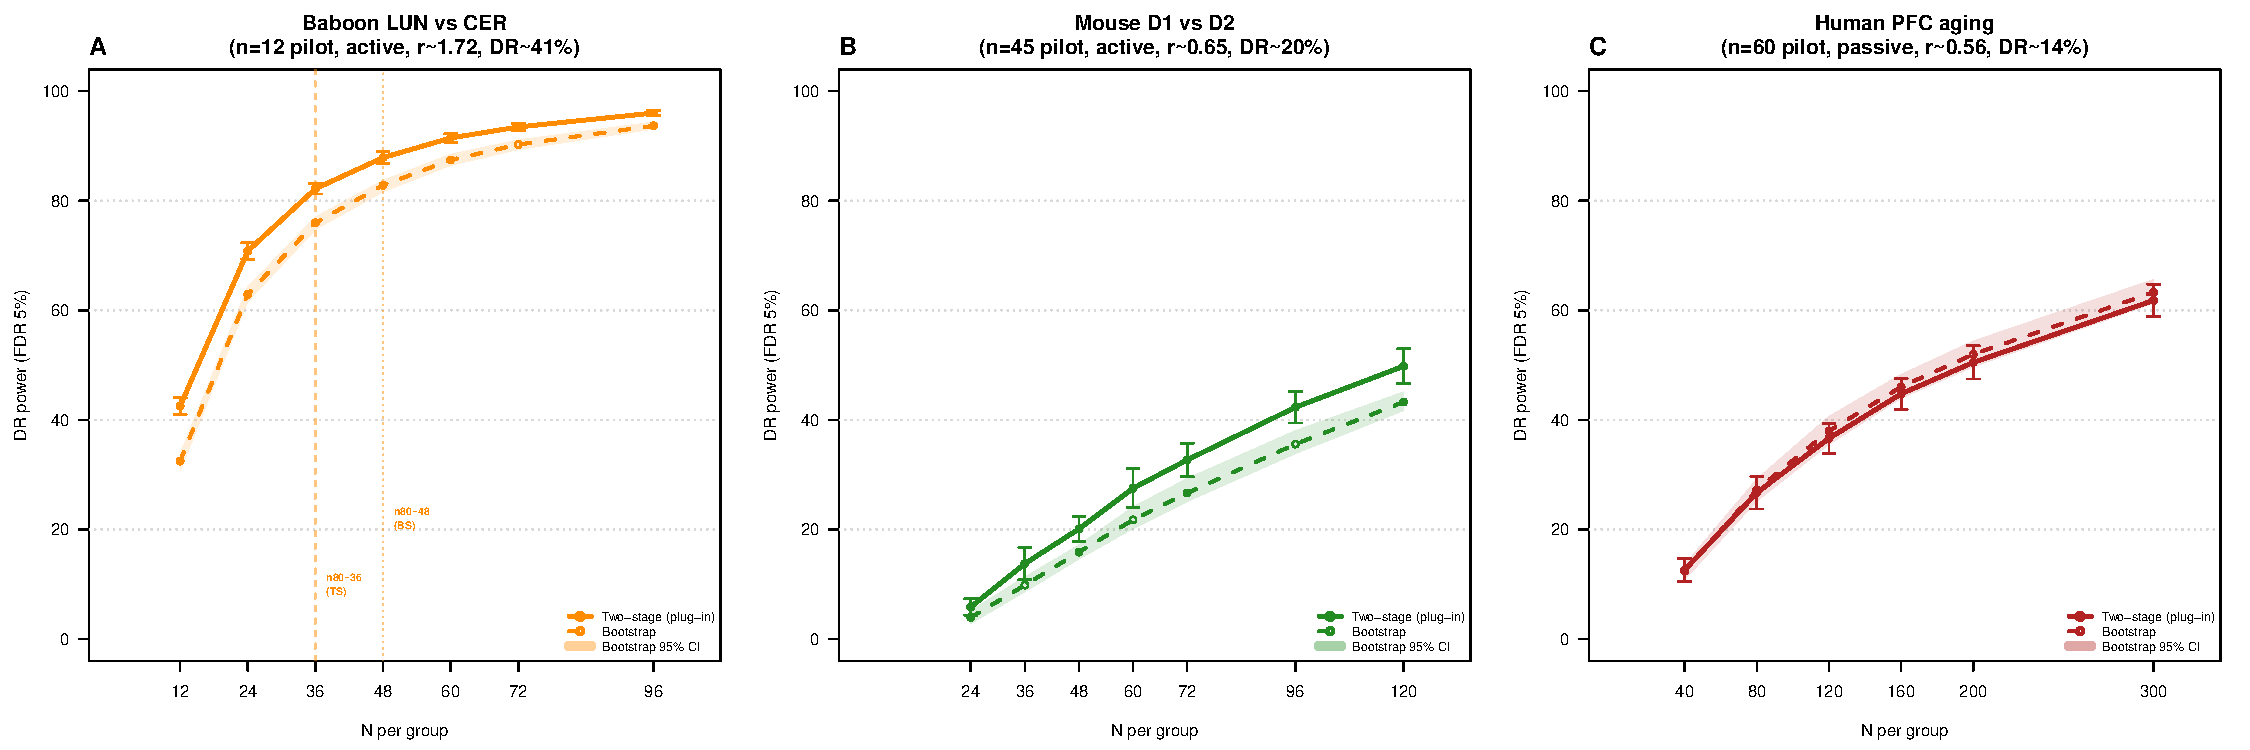
\includegraphics[width=\textwidth]{figures/bootstrap_summary.pdf}
\caption{Bootstrap vs.\ two-stage projected DR power across three pilot datasets.
Left: Baboon LUN vs.\ CER ($n=12$, active $B=12$, $m=1$).
Centre: Mouse D1 vs.\ D2 ($n=45$, active $B=6$).
Right: Seney MDD vs.\ Control ACC ($n=60$, passive).
Solid lines: two-stage plug-in power. Dashed lines: bootstrap mean power.
Shaded bands: 95\% bootstrap CI (pointwise). For Baboon, the plug-in
overestimates power by 5--7\,pp. CI width reflects pilot informativeness:
the active Baboon design ($B=12$, full 24\,h coverage) yields tighter
intervals than the passive Seney design despite a smaller pilot sample.}
\label{fig:bootstrap_baboon}
\end{figure}

\begin{figure}[H]
\centering
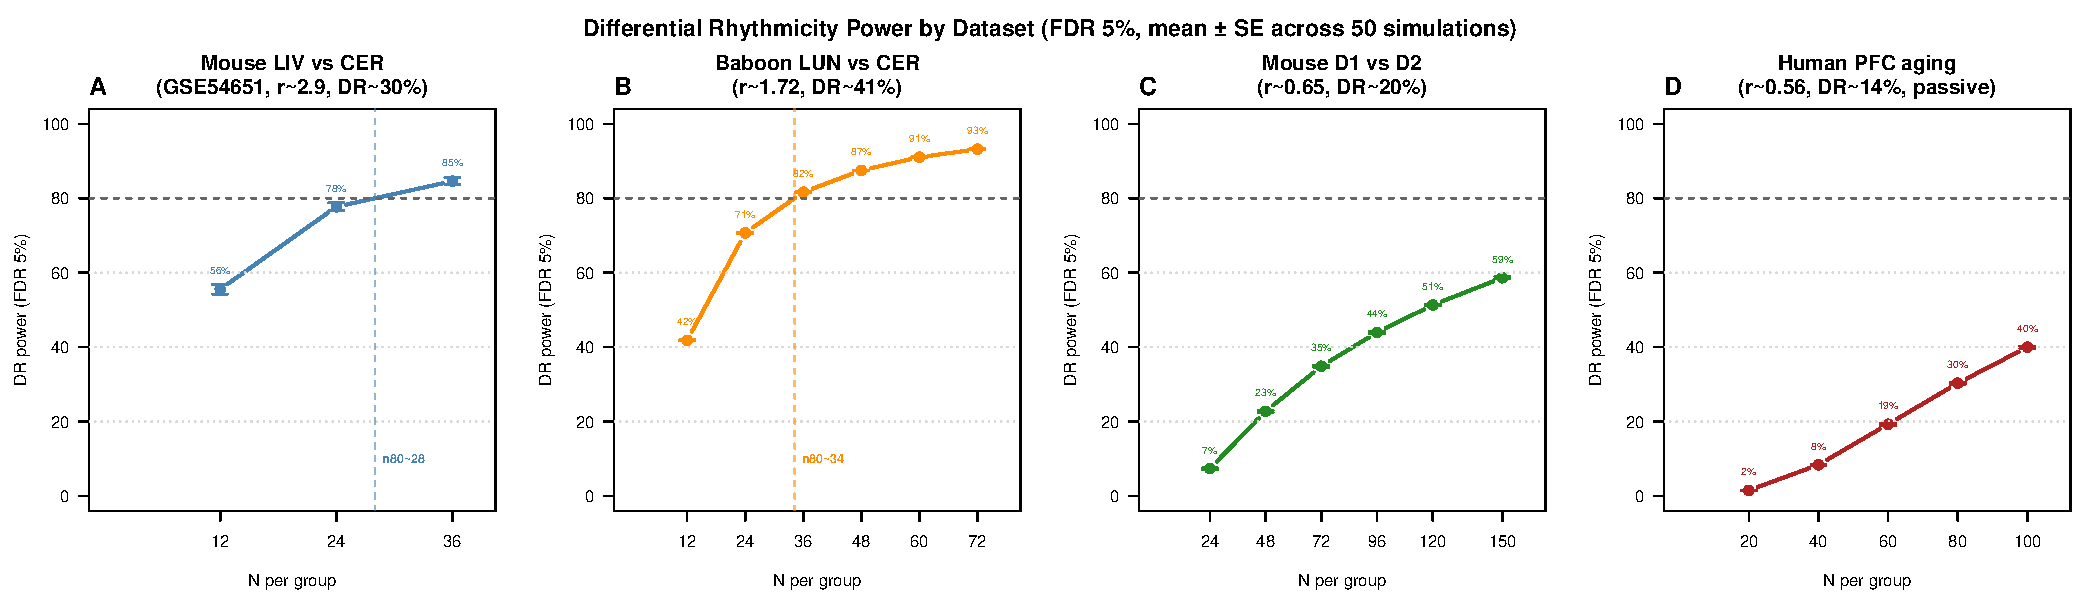
\includegraphics[width=\textwidth]{figures/multi_dataset_dr_power.pdf}
\caption{DR power vs.\ $N$ for four pilot datasets at FDR 5\% (mean $\pm$ SE across 50 simulations). Panels ordered by effect size (left to right: $\tilde{r} = 2.88$, $1.72$, $0.65$, $0.56$). Dashed line: 80\% power target. Vertical dashed line: interpolated $n_{80}$. The 5-fold range in $\tilde{r}$ translates to more than an order-of-magnitude difference in required sample size.}
\label{fig:multi_dr_power}
\end{figure}

\begin{figure}[H]
\centering

\includegraphics[width=\textwidth]{figures/bm_tradeoff.pdf}
\caption{B vs.\ m tradeoff across datasets (from left: Mouse LIV vs.\ CER, Baboon LUN vs.\ CER, Mouse D1 vs.\ D2). Each line is a $B$ value; shaded bands show 95\% bootstrap CIs. For the high-signal datasets (Mouse LIV, Baboon), $B$ and $m$ are approximately interchangeable for $B \geq 6$ (B-invariance holds). For the weak-signal D1D2 dataset, $B = 6$ substantially outperforms $B = 3$ at all $N$, demonstrating that denser temporal coverage is essential when $\tilde{r}$ is low.}
\label{fig:bm_tradeoff}
\end{figure}

\begin{figure}[H]
\centering
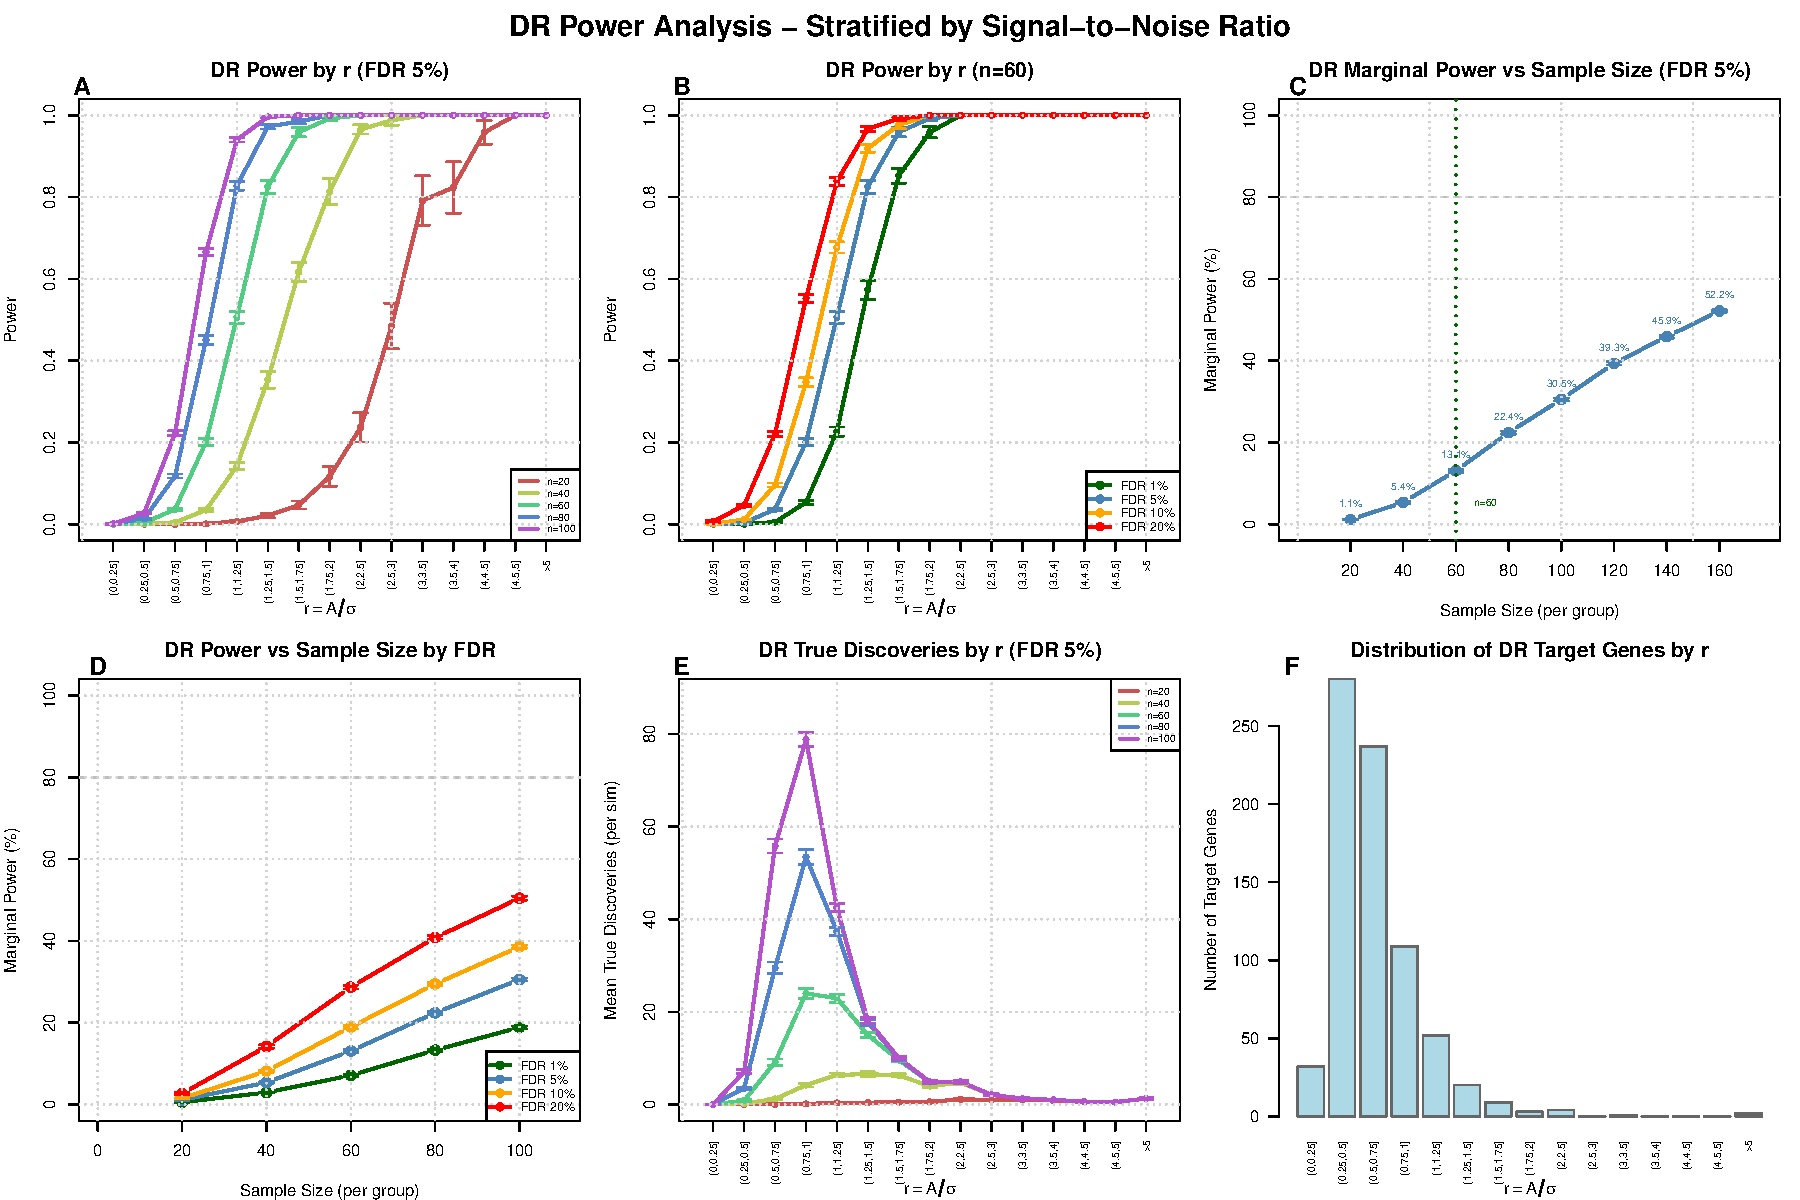
\includegraphics[width=\textwidth]{figures/dr_power.pdf}
\caption{DR power analysis. (A) Power by $r$ stratum at FDR 5\%. (B) Power by FDR threshold ($n=60$; sensitivity to nominal FDR). (C) Overall (marginal) per-gene power vs.\ sample size. (D) Overall (marginal) per-gene power by FDR threshold (sensitivity to nominal FDR). (E) True discoveries by $r$ stratum. (F) Empirical distribution of DR targets across $r$ strata.}
\label{fig:dr_power}
\end{figure}

\begin{figure}[H]
\centering
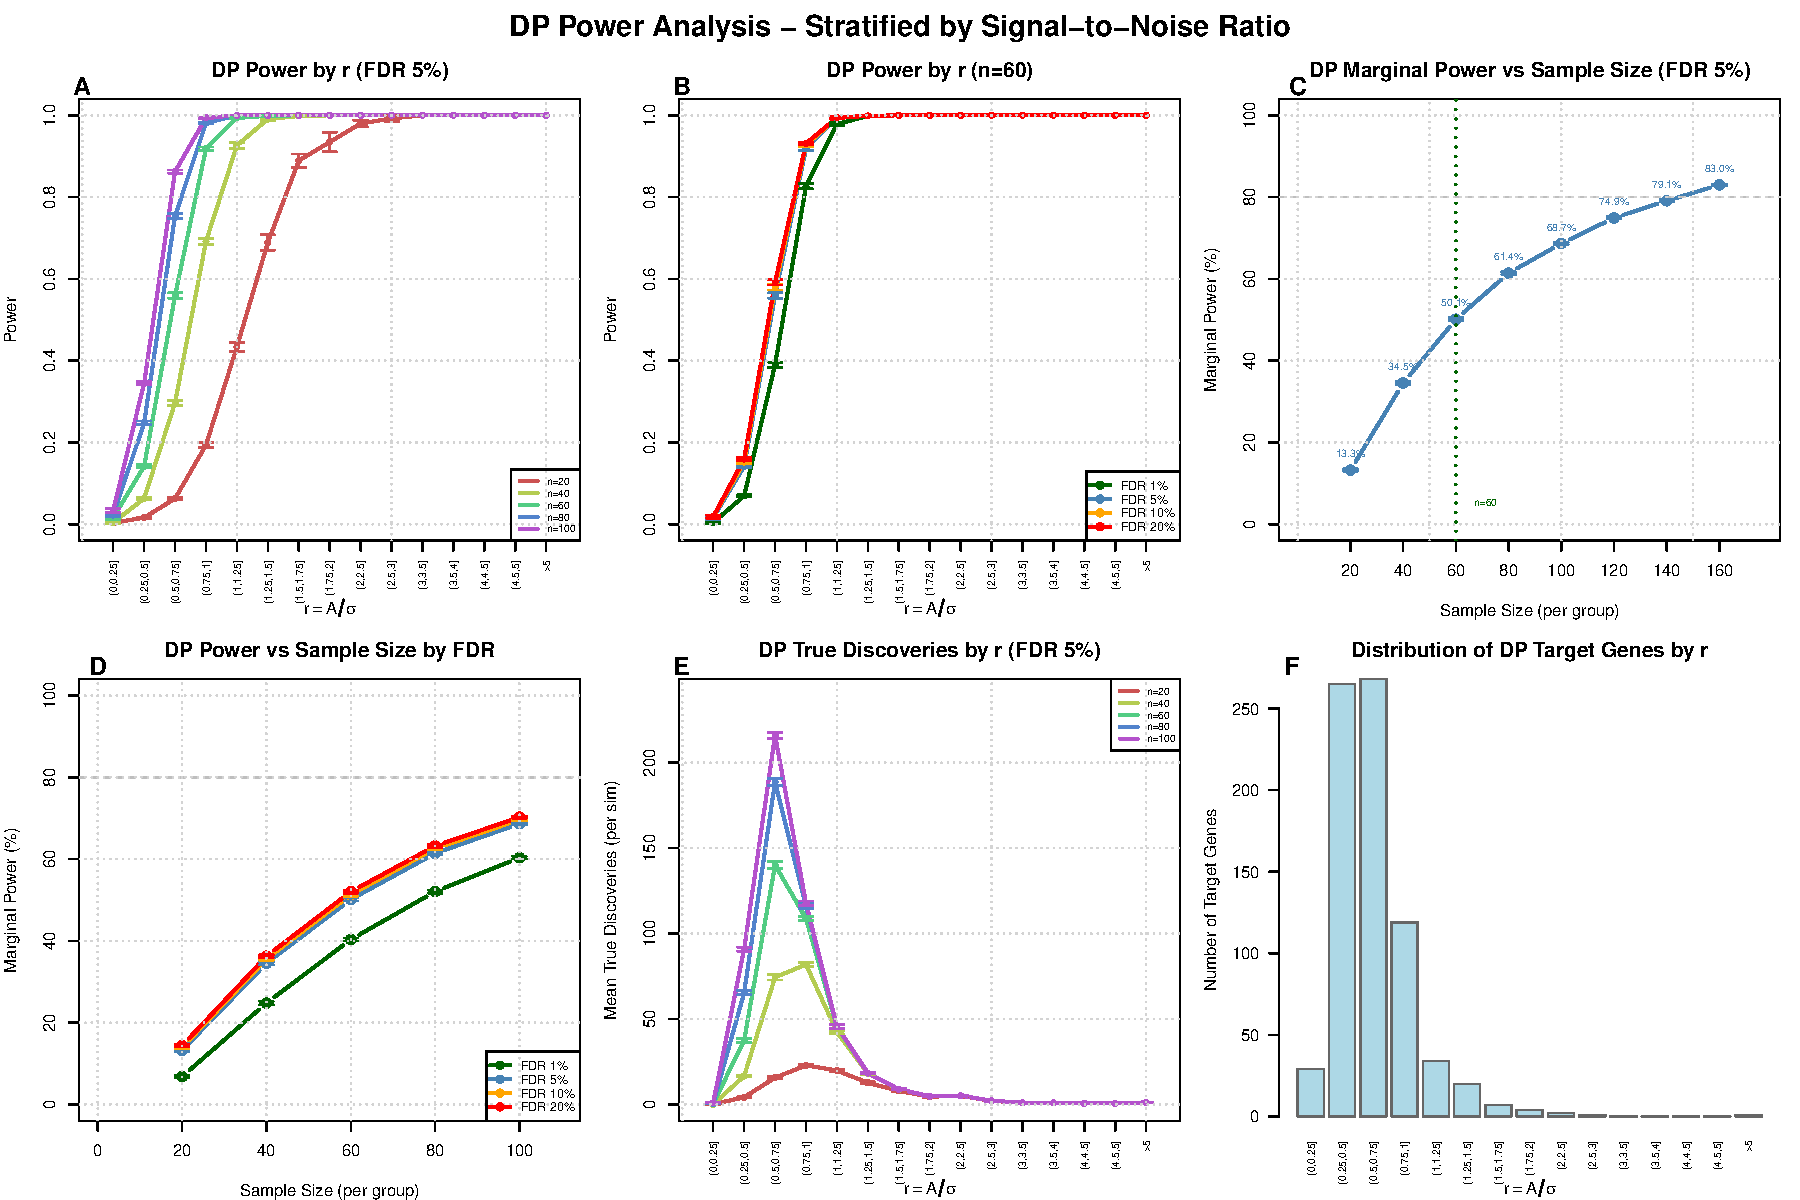
\includegraphics[width=\textwidth]{figures/dp_power.pdf}
\caption{DP power analysis ($\pm$6\,h phase shift). (B,D) show sensitivity to nominal FDR; (F) shows the empirical distribution of DP targets across $r$ strata. Panel layout otherwise matches Figure~\ref{fig:dr_power}.}
\label{fig:dp_power}
\end{figure}

\begin{figure}[H]
\centering
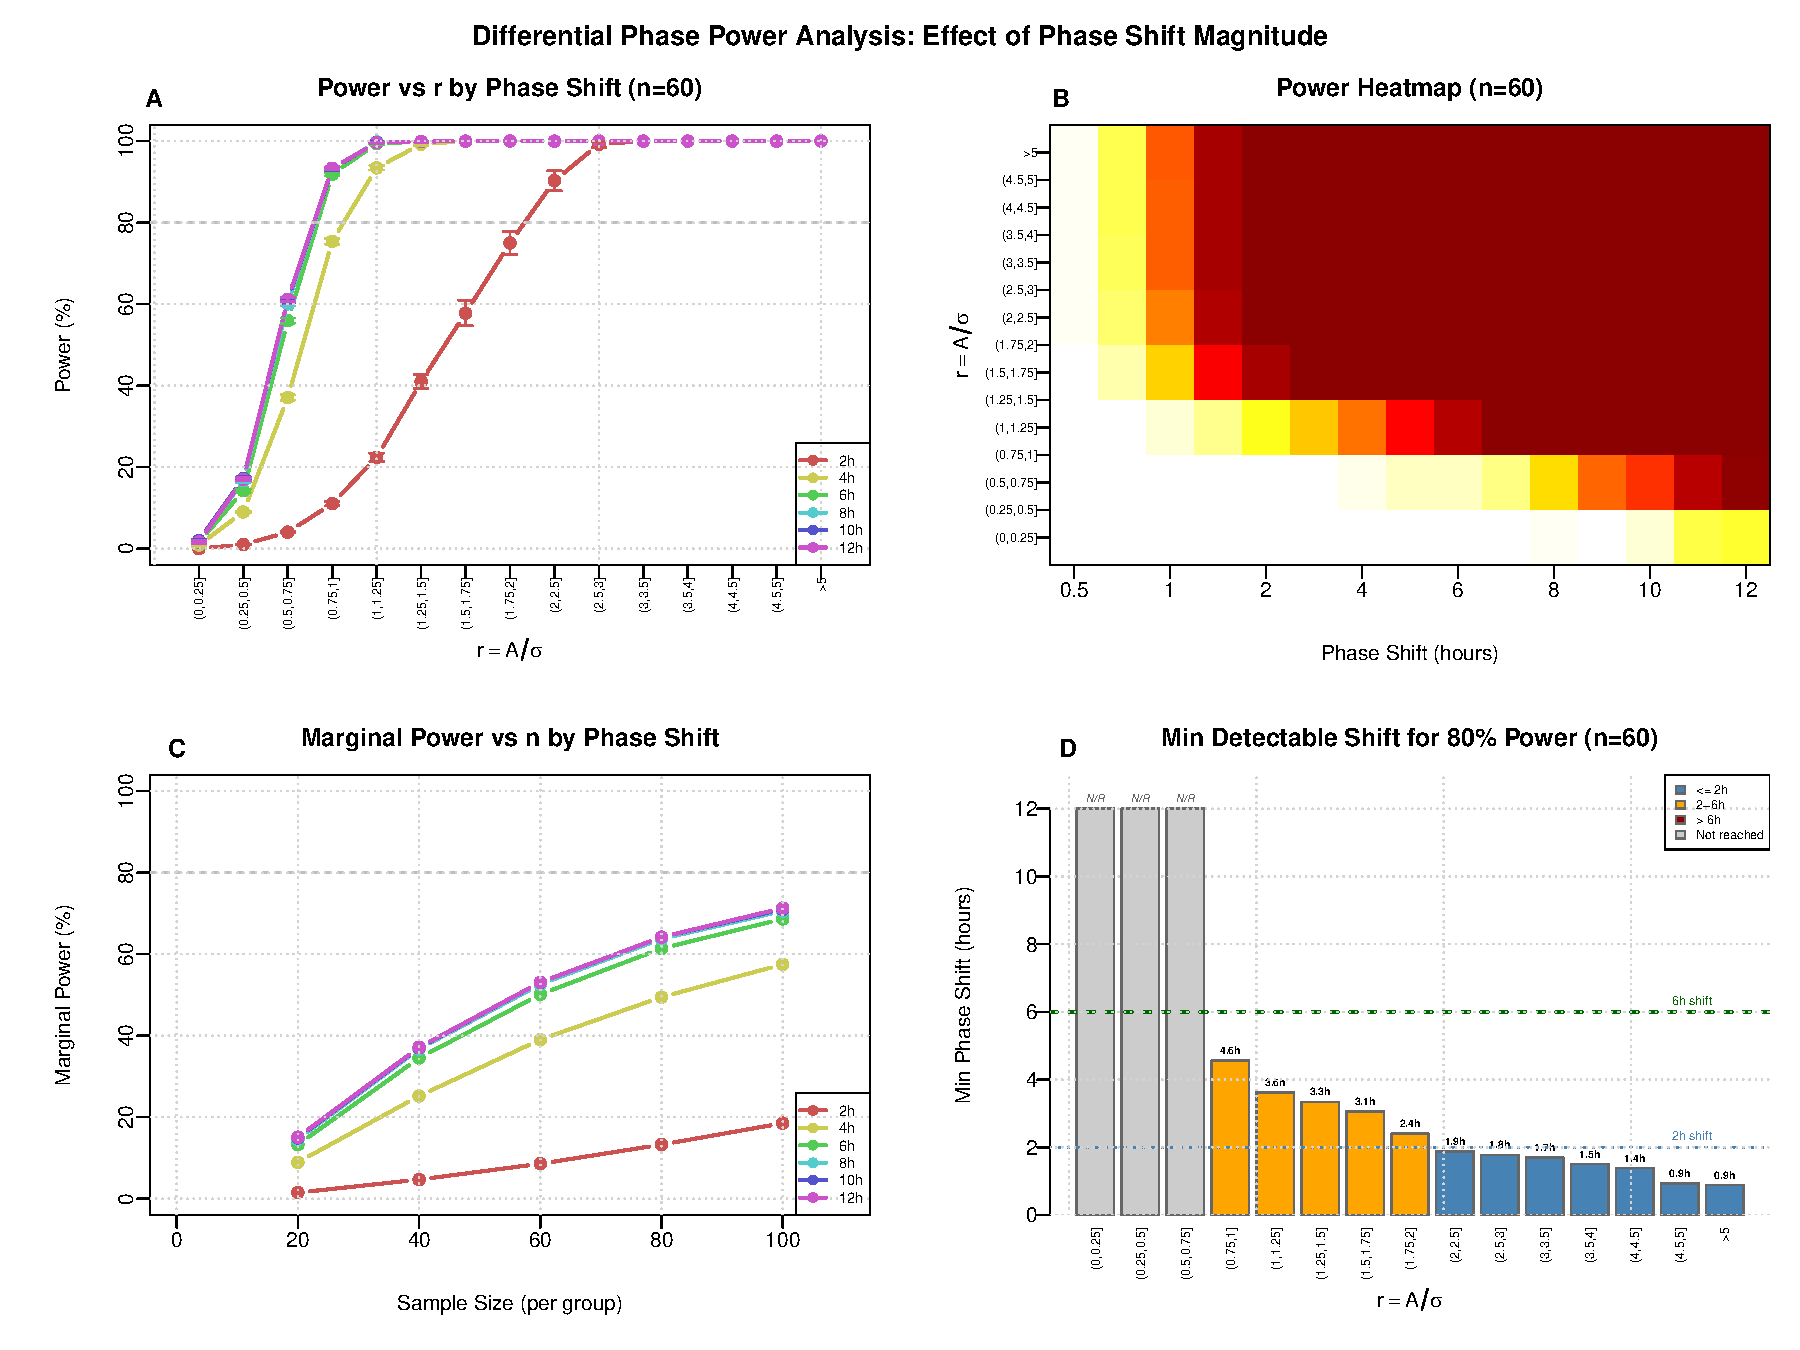
\includegraphics[width=\textwidth]{figures/phase_shift_abdf.pdf}
\caption{Phase shift sensitivity (5,000 genes, 50 simulations). (A) Power by $r$ stratum at $n=60$ across phase shifts. (B) Power heatmap ($r$ by phase shift). (C) Overall (marginal) per-gene power vs.\ sample size across phase shifts. (D) Minimum detectable phase shift by $r$ at $n=60$ (80\% power threshold).}
\label{fig:phase_shift_abdf}
\end{figure}

\begin{figure}[H]
\centering
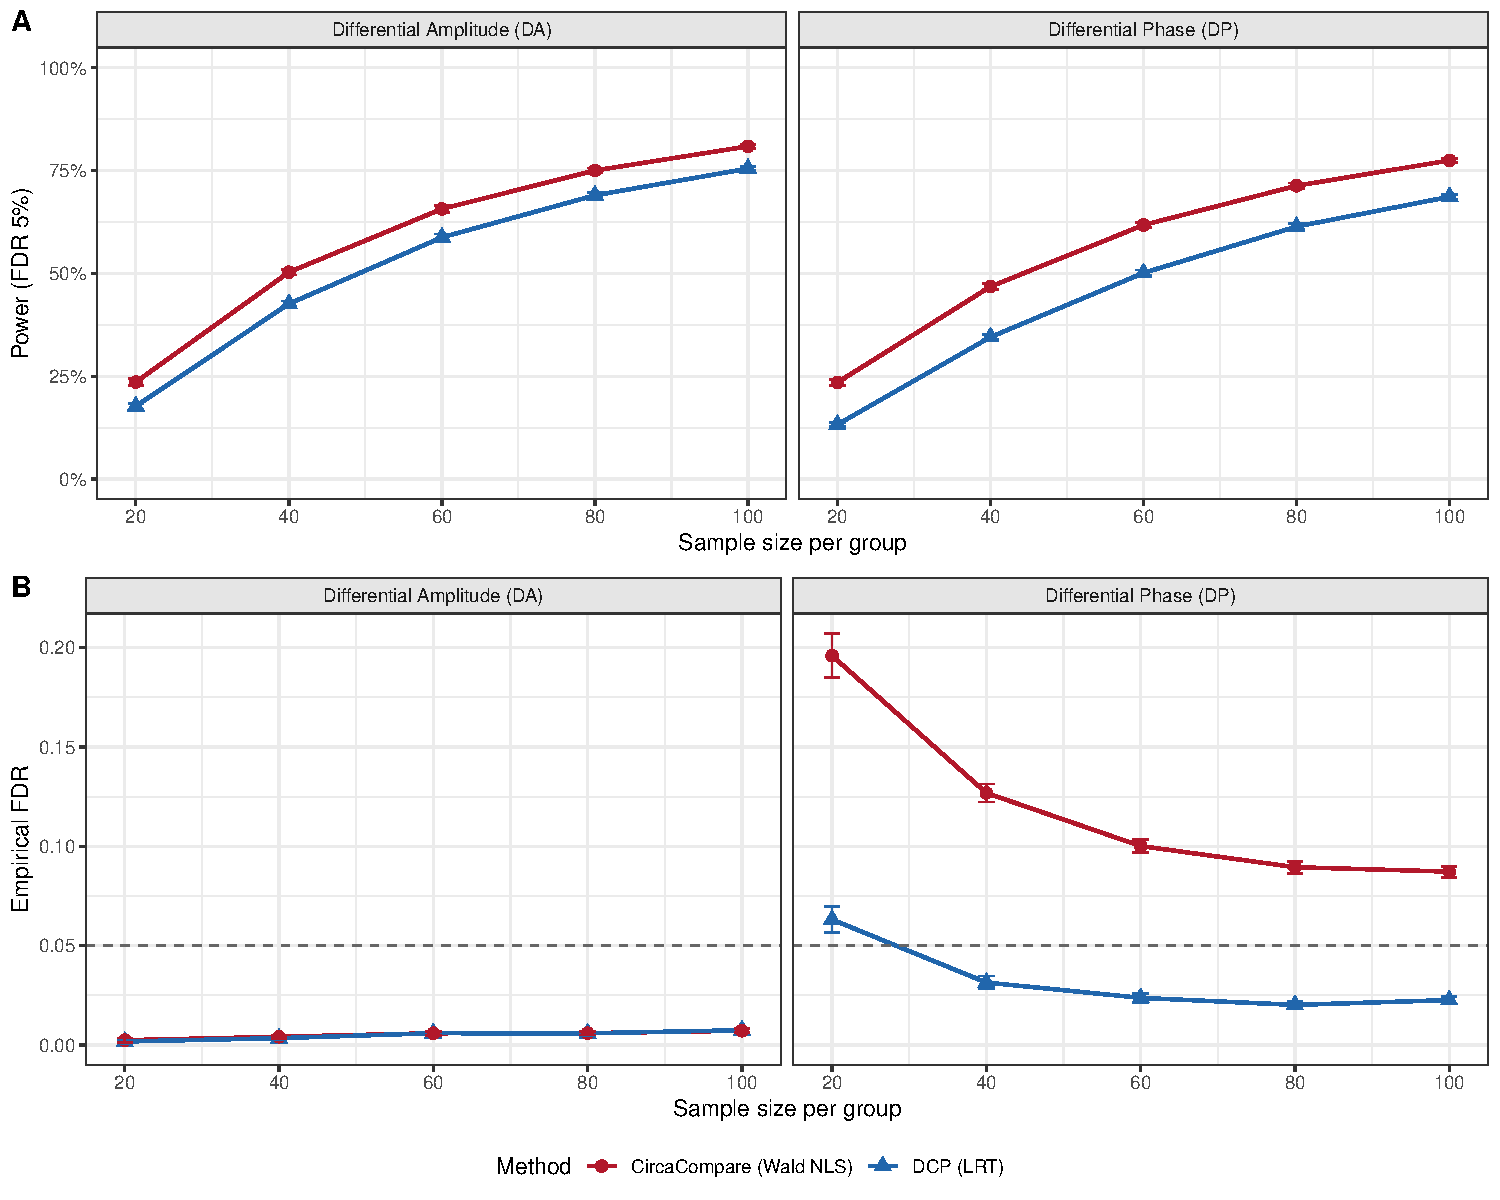
\includegraphics[width=\textwidth]{method_comparison/figures/method_comparison_combined.pdf}
\caption{Method comparison: DCP (LRT) vs.\ CircaCompare (Wald NLS) for DP. (A) Marginal power at FDR 5\%. CircaCompare achieves consistently higher power. (B) Empirical FDR. CircaCompare inflates empirical FDR to 8.7--19.6\%, far above the nominal threshold (dashed line), while DCP maintains proper control. Error bars show $\pm$1.96 SE across 50 simulations.}
\label{fig:method_comparison}
\end{figure}

\end{document}
